\documentclass[12pt,a4paper]{article}

\usepackage[utf8]{inputenc}
\usepackage[ngermanb]{babel}
% \usepackage{alphabeta} 
\usepackage{algpseudocode}
\usepackage{algorithm}

\usepackage[pdftex]{graphicx}
\usepackage[top=1in, bottom=1in, left=1in, right=1in]{geometry}

\linespread{1.06}
\setlength{\parskip}{6pt plus2pt minus2pt}
\setcounter{tocdepth}{3}

\widowpenalty 10000
\clubpenalty 10000

\newcommand{\eat}[1]{}
\newcommand{\HRule}{\rule{\linewidth}{0.5mm}}

\usepackage[official]{eurosym}
\usepackage{enumitem}
\setlist{nolistsep,noitemsep}
\usepackage[hidelinks]{hyperref}
\usepackage{cite}
\usepackage{svg}
\usepackage{amsfonts}
\usepackage{tikz}
\usetikzlibrary{shapes}

\setlength{\parindent}{0pt}
    
\floatname{algorithm}{Prozedur}

\usepackage{fancyhdr}
\pagestyle{fancy}
\cfoot{\thepage}
\lhead{InformatiCup2021}
\chead{Team \textit{Brot}}
\rhead{\nouppercase{\leftmark}}

\begin{document}

%===========================================================
\begin{titlepage}
\begin{center}

% Top 
%\includegraphics[width=0.4\textwidth]{Titel.jpg}~\\[1cm]


% Title
%\HRule \\[0.4cm]
%\vspace{0.4cm}
\vspace*{2cm}
{ \LARGE 
  \textbf{InformatiCup 2021 -- spe\_ed}\\[0.4cm]
  Theoretische Ausarbeitung\\
}
%\HRule \\[1.5cm]
\vspace*{3cm}

% Author
{ \large
  des Teams \\[0.5cm]
  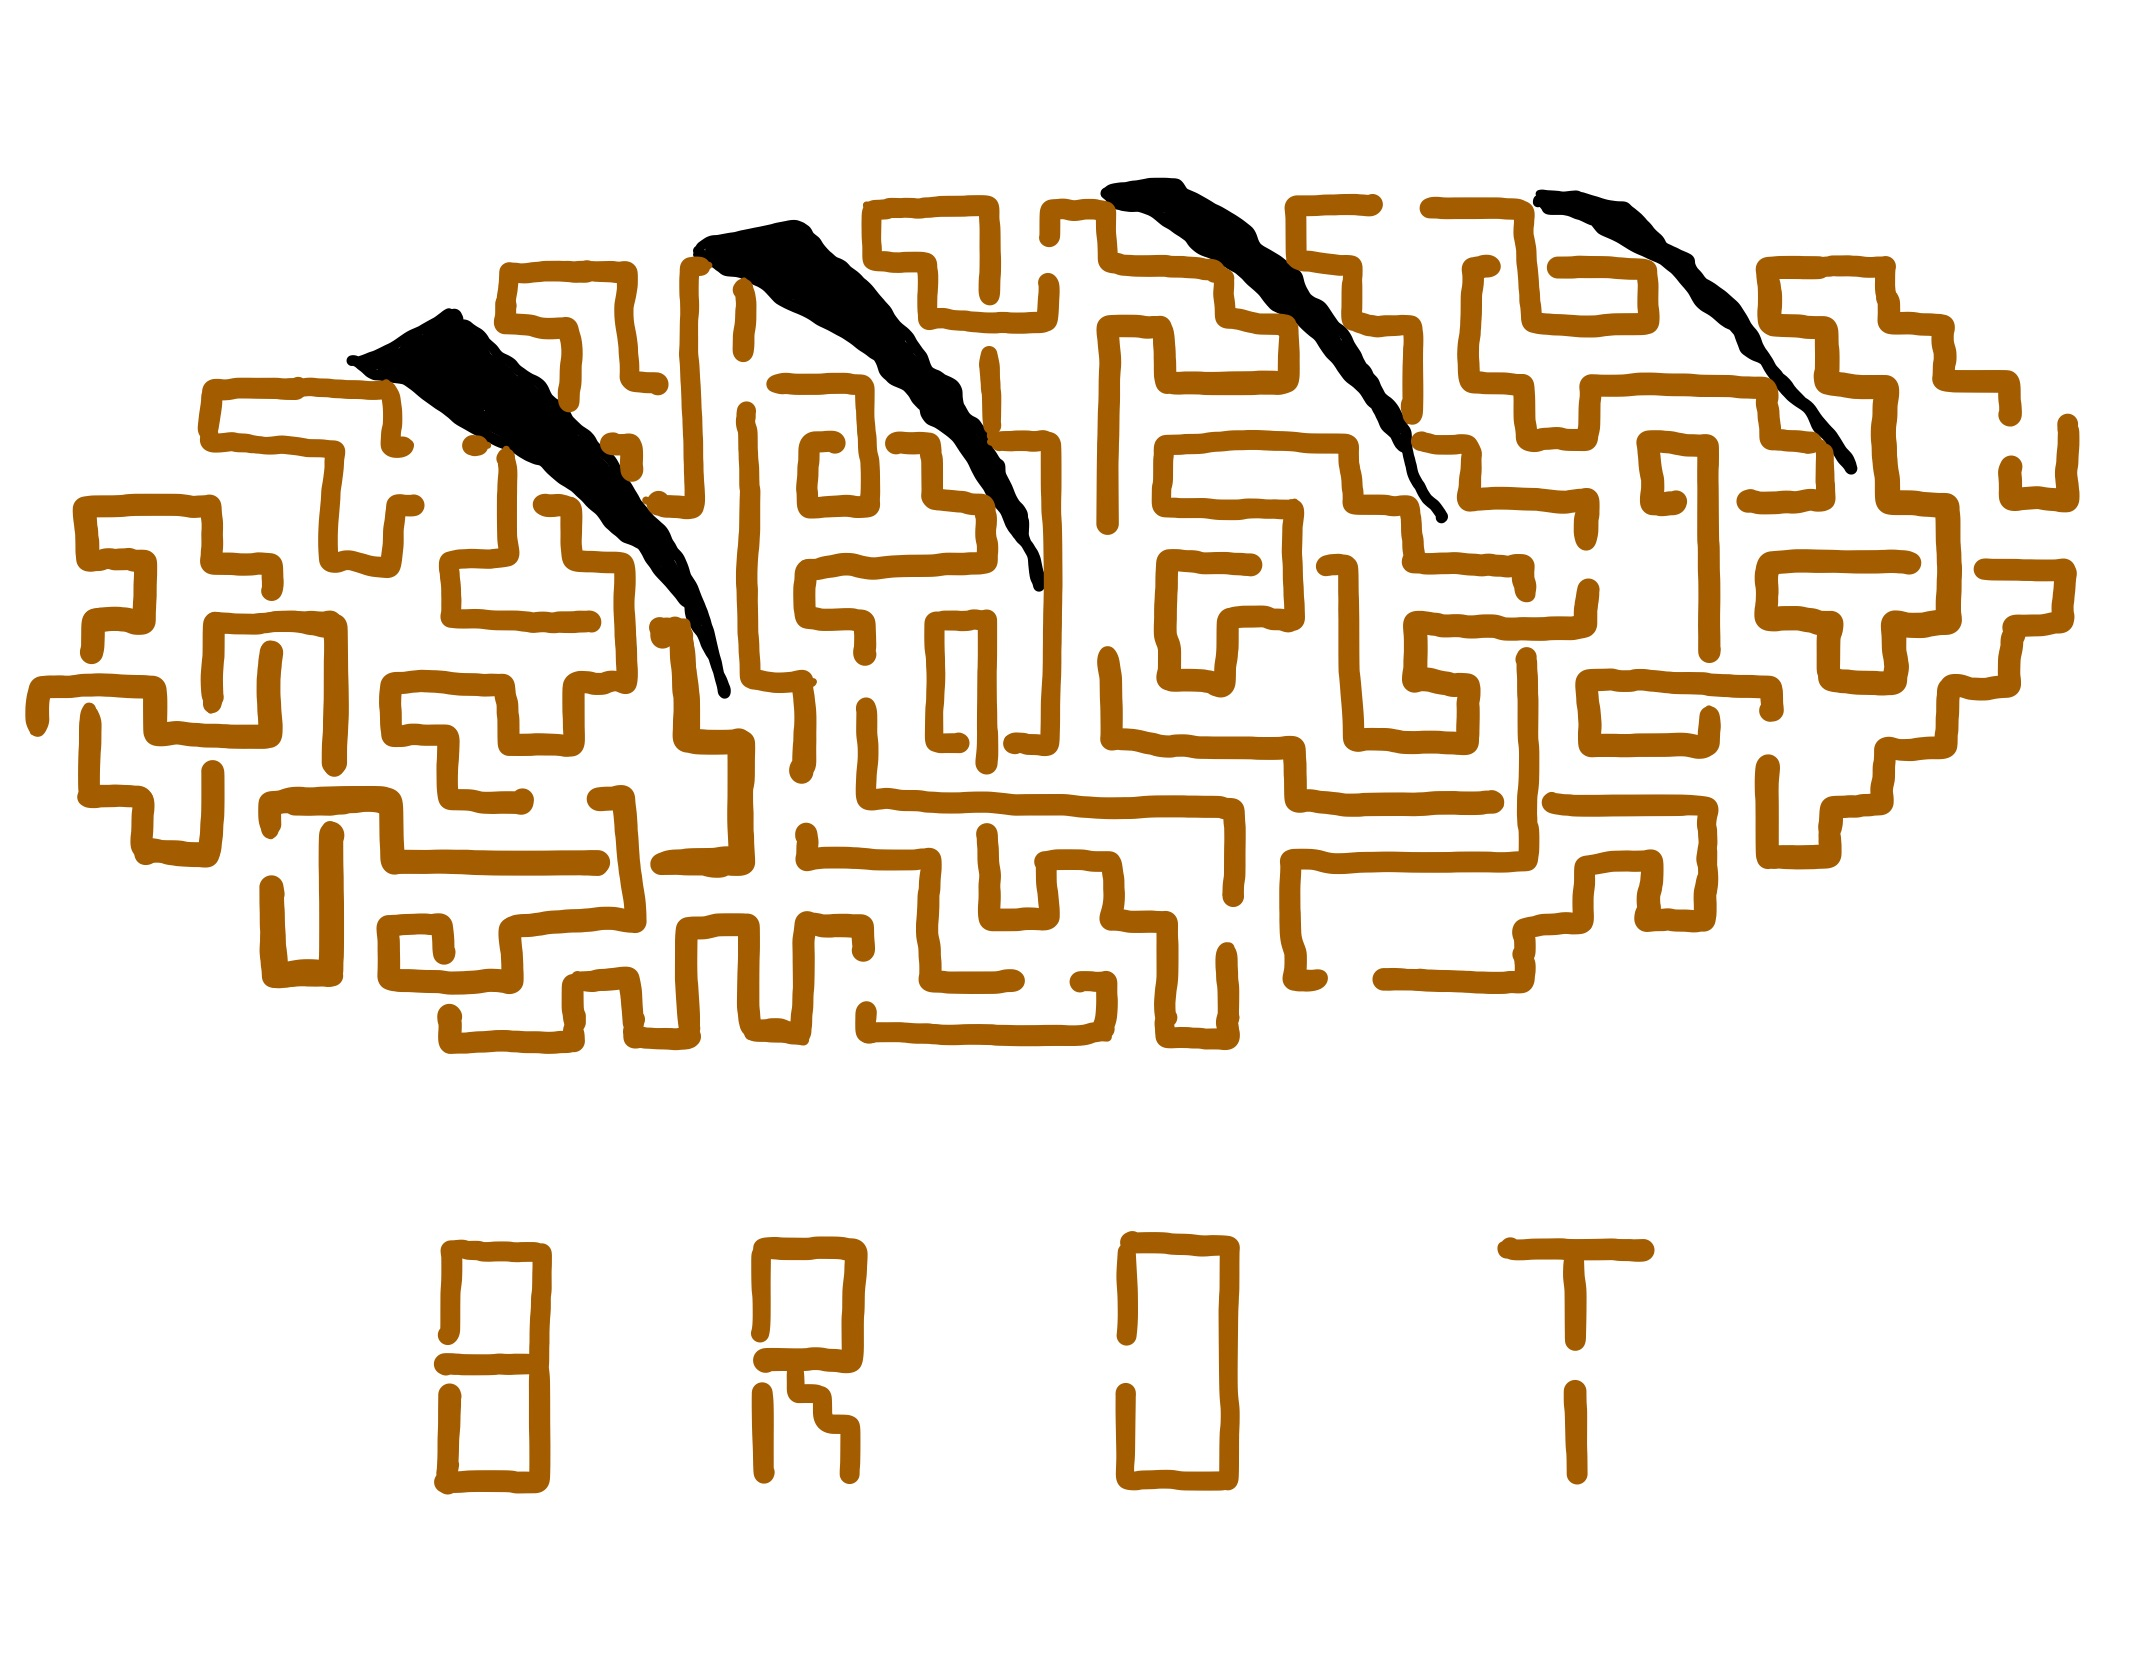
\includegraphics[width=0.3\textwidth]{brot_logo.jpg}~\\
  %\textit{Brot} \\[0.5cm]
  bestehend aus \\[3cm]
  Jacob Schäfer (\texttt{jacob.schaefer@student.hpi.de}), \\
  Alexander Sohn (\texttt{alexander.sohn@student.hpi.de}), \\
  Richard Wohlbold (\texttt{richard.wohlbold@student.hpi.de}), \\
  Lilly Zintl (\texttt{lilly.zintl@student.hpi.de}) \\
}
\vfill



% Bottom
{\large \today}
 
\end{center}
\end{titlepage}

%\begin{abstract}
%\lipsum[1-2]
\addtocontents{toc}{\protect\thispagestyle{empty}}
%\end{abstract}

\newpage



%===========================================================
\tableofcontents
%\addtocontents{toc}{\protect\thispagestyle{empty}}
\thispagestyle{empty}
\newpage

\listoffigures
\thispagestyle{empty}
\newpage

\setcounter{page}{1}

%===========================================================
%===========================================================

\section{Einleitung}
Beim InformatiCup 2021 ist die Aufgabe, ein Programm zu implementieren, welches das Spiel \texttt{spe\_ed} spielt. \texttt{spe\_ed} ist ein rundenbasiertes Spiel, bei dem alle Spieler gleichzeitig ziehen. Ein Spieler kann sich innerhalb eines Spielfelds bewegen und hinterlässt in jeder Zelle, die er überquert, eine Spur, die nicht verschwindet. Ein Spieler kann pro Runde einen Zug ausführen. Dabei hat er mehrere Möglichkeiten: Entweder geht er mit unveränderter Geschwindigkeit geradeaus, biegt nach links oder rechts ab oder ändert seine Geschwindigkeit um eins. Ein Spieler scheidet aus, wenn er versucht, eine Zelle zu betreten, die bereits von einem Spieler betreten wurde oder versucht, das Feld zu verlassen. Versuchen zwei Spieler, im selben Zug eine Zelle zu betreten, scheiden beide aus. Ziel des Spiels ist es, möglichst spät auszuscheiden. Zusätzlich gibt es die Mechanik des Springens: alle sechs Runden hinterlässt ein Spieler eine unvollständige Spur, sodass es ihm bei entsprechender Geschwindigkeit möglich ist, besetzte Zellen zu überspringen. Das Spiel findet gegen andere Teams auf einem Server statt. Die vollständige Aufgabenstellung kann im GitHub-Repository des InformatiCups (\texttt{https://github.com/informatiCup/\ InformatiCup2021}) eingesehen werden. In dieser Ausarbeitung erläutern wir die theoretischen Überlegungen und Ansätze für \texttt{spe\_ed} und gehen auf die konkrete Implementierung und Optimierung unserer Lösung ein. 

\section{Generelle Überlegungen}
Bei näherer Betrachtung der Spielregeln und der Aufgabenstellung fallen bereits einige Eigenschaften von \texttt{spe\_ed} auf, die bei der Entwicklung eines guten Programms, das in der Lage ist, \texttt{spe\_ed} zu spielen, (\textit{Client}) berücksichtigt werden müssen.

\subsection{Großer Verzweigungsfaktor}
Die hohe Anzahl an möglichen Spielzügen in jeder Runde führt zu einem hohen Verzweigungsfaktor. Der Verzweigungsfaktor beschreibt, wie viele Spielsituationen nach einem Zug aus einer Spielsituation entspringen können: Jeder Spieler hat in jedem Zug die Auswahl zwischen 5 verschiedenen Zügen. In einem Spiel, bei dem die maximale Anzahl von 6 Spielern erreicht wird, gibt es nach einem Zug bereits $5^6 = 15.625$ mögliche Folgesituationen. Eine Lösung durch Erstellen eines vollständigen Spielbaums ist also nicht sinnvoll. Es muss eine Spiellogik gefunden werden, die auf Grundlage verschiedener Kriterien sinnvoll Züge bewerten, vergleichen und ausschließen kann.


\subsection{Variable Parameter}
Die Rahmenbedingungen des Spiels sind sehr variabel. Weder die Deadline, bis zu der ein Spielzug abgegeben worden sein muss, noch die Größe des Spielfelds oder die Anzahl an Spielern ist genau festgelegt. Der Client darf also nicht zu rechenintensiv arbeiten, muss aber auch in unterschiedlichen Umgebungen gut funktionieren können.

\subsection{Gleichzeitiges Ziehen}
Auch das gleichzeitige Ziehen der Spieler erschwert die Wahl eines optimalen Zuges. Der Client weiß nicht, für welchen Zug sich die anderen Spieler in dieser Runde entscheiden und so kann ein Zug, der aktuell möglich scheint, doch zum Ausscheiden führen.

\subsection{Springen}
Die Möglichkeit des Springens muss bei einer sinnvollen Strategie berücksichtigt werden. Um diese Funktion einsetzen zu können, muss der Client über ein höheres Maß an Voraussicht verfügen, da der Sprung sowohl von der Anzahl an Zügen, als auch von der Geschwindigkeit des Spielers abhängt. Der Einsatz des Springens erweitert jedoch die Möglichkeiten und kann die Überlebenschancen erhöhen, sodass ein möglichst guter Client in der Lage sein sollte, diese Funktion sinnvoll einzusetzen.

\subsection{Hardwarevoraussetzungen und Netzwerklatenz}
Schwierigkeiten ergeben sich dadurch, dass die Hardwarevoraussetzungen nicht genau bekannt sind. So darf unsere Lösung nicht auf einer extrem rechenintensiven Strategie beruhen, die nur auf Systemen mit bestimmter, leistungsfähiger Hardware gute Ergebnisse liefert.

Es sollte zudem möglichst mit Strategien gearbeitet werden, die zu jeder Zeit ein Ergebnis vorweisen können, sodass die Rechenzeit genau an die Deadline angepasst werden kann. Ist dies nicht der Fall, wird entweder mögliche Rechenzeit verschwendet oder die Deadline verpasst, was zum Ausscheiden führen würde. 

Auch sollte aufgrund von Netzwerklatenz ein ausreichend großer Puffer eingeplant werden. Das Ergebnis muss schon vor der Deadline abgeschickt werden, da die Daten auch eine gewisse Übertragungszeit benötigen, um beim Server anzukommen. Es ist also wichtig, dass ein guter Mittelwert gefunden wird, bei dem immer noch möglichst viel Zeit für das Errechnen der Lösung, aber auch genug Puffer zum Senden der Daten bleibt.

\section{Verworfene Strategien}

\subsection{Einsatz einer einfachen Logik}
Um uns dem Thema anzunähern, haben wir zunächst einen sehr einfachen Client implementiert. Dieser soll später außerdem als Referenz dienen, um die Qualität anderer Ansätze bewerten zu können. Der \textit{Basic-Client} betrachtet zunächst, welche Züge aktuell für ihn möglich sind, d.h. welche Züge er momentan ausführen kann, ohne zu sterben. Immer wenn der Client geradeaus gehen kann, wird dies als Zug gewählt. Ansonsten versucht er nach links zu gehen. Falls dies auch nicht möglich ist, biegt er rechts ab.

Der Basic-Client abstrahiert das Spielgeschehen sehr stark. Er berücksichtigt nicht, dass alle Spieler gleichzeitig ziehen, ändert nie seine Geschwindigkeit und springt daher auch nicht. Außerdem betrachtet der Basic-Client immer nur den aktuellen Zug und ist nicht in der Lage, Züge vorauszuplanen. Deshalb schlägt er oft Wege ein, die eine sichere Kollision mit der Wand bedeuten, indem er beispielsweise in Sackgassen läuft, wie in Abbildung \ref{fig:smart-dead} zu sehen ist.

\begin{figure}[h]
    \centering
    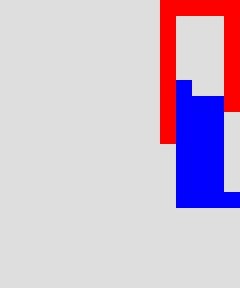
\includegraphics[width=0.4\textwidth]{smart.jpg}
    \caption{Der Basic-Client (rot) erkennt nicht, dass er in eine Sackgasse läuft}
    \label{fig:smart-dead}
\end{figure}

\subsection{Monte-Carlo-Tree-Search}
Monte-Carlo-Tree-Search (MCTS) ist ein Verfahren, das sich der optimalen Lösung an\-nähert, indem der Spielbaum stichprobenartig durchsucht und aufgebaut wird. Durch die Anwendung von Heuristiken können eine höhere Suchtiefe erreicht und vielversprechendere Bereiche des Entscheidungsbaums betrachtet werden \cite{browne2012}.

MCTS versucht beim Aufbau des Spielbaums eine Balance zwischen \textit{Exploration}, dem Untersuchen bisher wenig untersuchter Bereiche des Baums und \textit{Exploitation}, dem weiteren Untersuchen vielversprechender Teile des Baums, zu finden \cite{browne2012}. 

Der Wurzelknoten des Spielbaums ist der aktuelle Spielzustand. Um mit diesem Verfahren den Spielbaum aufzubauen, werden folgende Phasen durchlaufen:
\begin{enumerate}
    \item{\textit{Selektion}:} Es wird, beginnend beim obersten Knoten des Baumes, immer der vielversprechendste Knoten ausgewählt, bis dieser keine Nachfolger mehr hat.
    \item{\textit{Expansion}:} Ausgehend von diesem Knoten werden alle möglichen Spielzüge ausgeführt und jeweils der daraus resultierende Spielzustand als Knoten gespeichert.
    \item{\textit{Simulation}:} Ausgehend von diesen Spielzuständen werden komplette Spiele mit zufälligen Zügen simuliert, sogenannte \textit{Rollouts}. Der jeweilige Spielzustand wird anschließend anhand der durch die Rollouts gewonnenen Erkenntnisse bewertet. Ein Bewertungskriterium kann zum Beispiel die Gewinnrate sein.
    \item{\textit{Rückwärtspropagierung}:} Mit den Ergebnissen der Rollouts wird der komplette Spielbaum aktualisiert.
\end{enumerate}
In der Selektionsphase wird eine Metrik benötigt, um herauszufinden, welcher Knoten in der nächsten Ebene am vielversprechendsten ist. Eine Lösung liefert der UCT (Upper Confidence Bound applied to trees)-Algorithmus. Dieser setzt Exploration und Exploitation ins Verhältnis und gewichtet zwischen diesen. Dabei wird für jeden möglichen Zug der folgende Ausdruck ausgewertet und anschließend maximiert:

\[ \frac{w_i}{n_i}+c \cdot \sqrt{\frac{\ln N_i}{n_i}} \]

Dabei steht $w_i$ für die Anzahl an gewonnenen Spielen nach Zug $i$, $n_i$ für die Anzahl an Simulationen, die für diesen Knoten nach dem $i$-ten Zug ausgeführt wurden und $N_i$ für die Anzahl an Simulationen, die für den Elternknoten ausgeführt wurden. $c$ ist ein fester Wert, der zwischen Exploitation und Exploration gewichtet und für das jeweilige Spiel bestimmt werden muss \cite{kocsis2006}. 

In dieser Formel steht der erste Teil für die Exploitation: Je öfter nach einem Knoten Spiele gewonnen wurden, desto höher ist das Verhältnis zwischen gewonnen Spielen und Simulationen. Der zweite Teil setzt die eigene Besuchshäufigkeit mit der des Elternknotens in Beziehung. Dabei werden Knoten, die im Vergleich zum Elternknoten weniger häufig besucht wurden, bevorzugt.

Die Metrik jedes Knotens wird immer mit den Ergebnissen aus den Rollouts aktualisiert. Dies nennt man \textit{Rückwärtspropagierung}. Dabei werden beginnend vom aktuellen Knoten bis zum Wurzelknoten die Besuchshäufigkeiten und die Gewinnrate entsprechend aktualisiert. Dadurch ergibt sich auch für jeden Knoten ein neuer Wert der Metrik. Nach der Rückwärtspropagierung beginnt der Ablauf wieder mit der Selektionsphase.

Nach einer möglichst hohen Anzahl an Durchläufen gilt der Knoten in der ersten Expansionsebene mit der größten Besuchshäufigkeit als am vielversprechendsten.

\subsubsection{Vorteile}
Das beschriebene Verfahren hat für \texttt{spe\_ed} insbesondere einen wichtigen Vorteil: Da das Bewertungskriterium während der gesamten Berechnung vorliegt, kann zu jedem Zeitpunkt ein bis dahin bester Zug ermittelt werden. Somit kann bei diesem Verfahren die vorliegende Berechnungszeit vollständig genutzt werden.

\subsubsection{Nachteile}
Allerdings ergeben sich bei der Umsetzung von MCTS diverse Schwierigkeiten. Insbesondere die Eigenschaft, dass alle Spieler gleichzeitig ziehen, bewirkt, dass ein einzelner Zug nicht auf die herkömmliche Art und Weise bewertet werden kann. Je nach Anzahl der verbleibenden Spieler entstehen bis zu \(5^5 = 3125\) neue Spielsituationen pro Zug. Diese können zwar alle mithilfe von Rollouts bewertet werden, welche konkrete Spielsituation davon eintritt, hängt jedoch auch von den Zügen der anderen Spieler ab. Es würden also immer diejenigen Knoten favorisiert, die für gegnerische Spieler schlecht sind. Allerdings kann nicht angenommen werden, dass diese Züge auch von den Gegnern gewählt werden. Damit ist das Konzept von MCTS in diesem Fall nur schwierig anwendbar.

Um vorerst trotzdem nach dem herkömmlichen Schema vorgehen zu können, haben wir nur Spielsituationen berücksichtigt, welche auf möglichen Zügen der Spieler basieren. Zudem haben wir die Anzahl an berücksichtigten Spielern eingeschränkt. So erzielten wir einen durchaus spielfähigen Algorithmus. Durch die starke Vereinfachung bei der Expansion entstand jedoch auch eine hohe Unzuverlässigkeit und viele Züge der gegnerischen Spieler wurden nicht beachtet. So kam es beispielsweise oft zu der Situation, dass zwei Spieler in dieselbe Zelle ziehen wollten und infolgedessen beide verloren.

\subsubsection{Fazit} 
Wir haben also festgestellt, dass MCTS nach herkömmlicher Implementierung für das Spiel \texttt{spe\_ed} eher ungeeignet ist. Es wäre allerdings denkbar, dass der Algorithmus durch weitere Überlegungen durchaus verbessert werden kann. Obwohl wir diesen Ansatz verworfen haben, konnten wir dennoch die wichtige Erkenntnis gewinnen, dass Spielzustände mithilfe von Rollouts einigermaßen effizient und zuverlässig bewertet werden können.

\subsection{Reinforcement Learning}
Beim Reinforcement Learning wird ein Spieler (\textit{agent}) anhand seiner ausgeführten Züge (\textit{actions}) entweder belohnt oder bestraft. Wir betrachten dabei das Spielfeld zum Zeitpunkt $t$, das sich im Zustand (\textit{state}) $s_t$ befindet. Der Spieler (\textit{agent}) führt nun eine \textit{action} $a_t$ aus, die das Spielfeld von $s_t$ in $s_{t+1}$ überführt. Dafür erhält der Spieler einen \textit{reward} $r_t$. Da der \textit{agent} stets seinen zukünftigen \textit{reward} maximiert, entwickelt der \textit{agent} auf diese Art und Weise eigenständig eine sinnvolle Strategie für das Spiel. Eine Art des Reinforcement Learnings ist das Q-Learning \cite{schwaiger2019}.

Beim Q-Learning wird mittels der sog. Q-Funktion (Q für \textit{quality}) berechnet, wie vielversprechend eine \textit{action} $a$ im aktuellen Zustand $s_t$ ist. Hierzu werden zunächst 2 Tabellen angelegt. Zum einen ist das die R-Tabelle, die festlegt, für welche Ereignisse der Spieler welche Belohnung $r_t$ erhält (R für \textit{reward}). Ein Ereignis könnte hierbei zum Beispiel darstellen, wenn der Spieler in eine Wand läuft, was mit einem negativen \textit{reward} verknüpft wird. Zum anderen ist das die Q-Tabelle, die für die Paare $(s_t, a_t)$ den Wert der Q-Funktion speichert. Die Q-Tabelle wird zunächst mit dem Wert 0 initialisiert und später während des Spielens ständig mit den Spieldaten aktualisiert.

Innerhalb eines Spieles wird immer folgender Ablauf durchgeführt:
\begin{enumerate}
    \item Auswahl und Ausführen einer Aktion
    \item Ermitteln der Belohnung $r_t$
    \item Anpassen der Q-Tabelle
\end{enumerate}
Das Auswählen einer Aktion ist zu Beginn, wenn der Großteil der Q-Tabelle noch mit Nullen gefüllt ist, nicht eindeutig. Deshalb wird ein $\varepsilon$-Wert eingeführt, der zwischen 0 und 1 liegt und zu Beginn des Spiels sehr gering ist. Bei jedem Zug wird eine zufällige Zahl ermittelt. Wenn diese größer als $\varepsilon$ ist, wird aus allen möglichen \textit{actions} eine Zufällige ausgewählt. Da $\varepsilon$ mit jedem Zug erhöht wird, ist die Wahrscheinlichkeit, dass zu Beginn einfach zufällige Züge ausgeführt werden recht hoch. Später, wenn die Q-Tabelle dann etwas aussagekräftiger ist, wird die Wahrscheinlichkeit zufälliger Züge zunehmend geringer. Dann wird jeweils die Aktion mit dem höchsten Wert in der Q-Tabelle, also die vielversprechendste Aktion, ausgeführt. Der $\varepsilon$-Wert führt dadurch auch zu einem Übergang von \textit{Exploration} zu \textit{Exploitation}. Zu Beginnen werden die Züge eher zufällig gewählt, sodass noch unbekannte \textit{actions} ausgeführt und bewertet werden können, während später vor allem die Aktionen gewählt werden, die bereits gut bewertet wurden. 

Nachdem ein Zug gewählt und ausgeführt wurde, kann die Belohnung für diesen mittels der R-Tabelle bestimmt werden. Im dritten Schritt soll nun die Q-Tabelle mithilfe der folgenden Q-Funktion angepasst werden:
$$Q_{\mathrm{neu}}(s_t,a_t)=Q_{\mathrm{alt}}(s_t,a_t)+\alpha*(r_t+\gamma*\max Q(s_{t+1},a)-Q_{\mathrm{alt}}(s_t,a_t))$$
Um den neuen Q-Wert $Q_{\mathrm{neu}}(s_t,a_t)$ zu bestimmen, werden verschiedene Faktoren einbezogen:

\begin{itemize}
    \item $Q_{\mathrm{alt}}(s_t,a_t)$, ist der Wert, der aktuell für das Paar $(s_t,a_t)$ in der Q-Tabelle zu finden ist.
    \item $\alpha$ ist die sogenannte Lernrate. Diese hat i.d.R. einen Wert zwischen 1 und 0 und bestimmt wie drastisch die Q-Tabelle verändert wird. Liegt der Wert z.B. bei $\alpha =0$ würde gar keine Aktualisierung stattfinden.
    \item $r_t$ beschreibt die Belohnung, die der Spieler für den letzten Zug erhält.
    \item $\max Q(s_{t+1},a)$ beschreibt den maximalen Q-Wert für alle nächsten möglichen \textit{actions}. Hierfür werden alle Aktionen betrachtet, die im nächsten Zustand $s_{t+1}$ ausgeführt werden können und der höchste Q-Wert wird ausgewählt.
    \item $\gamma$ liegt zwischen 0 und 1 und beschreibt, wie stark die Bewertung der zukünftig möglichen Spiele mit $\max Q$ in $Q_{\mathrm{neu}}$ einfließen soll.
\end{itemize}

$Q_\mathrm{neu}$ wird also anhand der erhaltenen Belohnung aus dem letzten Zug sowie der Vermutung, wie vielversprechend der nun aktuelle Zustand $s_{t+1}$ für das weitere Spielgeschehen ist, bestimmt. So ist der \textit{agent} in der Lage, langfristig sinnvolle Entscheidungen zu treffen. Weiterhin ermöglicht der Ansatz, dass der Client mit jedem Spiel dazulernen und sich verbessern kann, denn die Q-Tabelle wird gespeichert und kann so bei jedem Spiel erweitert werden.

Aus diesem Grund führten wir eine erste Implementierung eines Q-Learning Clients durch. Als Zustand $s$ verwendeten wir dazu einen $n*n$ Zellen großen Spielfeldausschnitt um die aktuelle Position des Spielers herum. Dieser Ausschnitt wurde als zweidimensionales Array implementiert, wobei die entsprechenden Elemente für freie Zellen auf 0 und für besetzte Zellen auf 1 gesetzt wurden. Den Ansatz, das gesamte Spielfeld zu betrachten, verwarfen wir direkt aufgrund der großen Menge an Spielfeldzuständen. Diese müssten nämlich zum einen alle einen separaten Eintrag in der Q-Tabelle erhalten und zum anderen wäre eine Q-Tabelle dann nur schwer für mehrere Spiele nutzbar, da die Spielfeldgröße bei \texttt{spe\_ed} variabel ist. Bei Betrachtung der Ergebnisse stellten wir jedoch fest, dass die Nutzung von Q-Learning auch einige Nachteile mit sich brachte.

\subsubsection{Nachteile}
Das größte Problem stellte dabei immer noch die zu große Anzahl an möglichen Spielfeldzuständen dar. Außerdem muss der Client nach jeder Parameteränderung zunächst eine längere Trainingsphase durchlaufen, bevor die Qualität des Spielers sinnvoll bewertet werden kann, da die neue Q-Tabelle erst wieder aufgefüllt werden muss. Weiterhin wird bei diesem Ansatz, auch nicht beachtet, dass alle Spieler gleichzeitig Ziehen, wodurch die bereits beschriebenen Probleme auftreten können.

\subsubsection{Fazit}
Auch wenn unsere Implementierung von Q-Learning noch Verbesserungspotential hatte, entschieden wir uns aufgrund der genannten Probleme, diesen Ansatz nicht weiter zu verfolgen.

\section{Verwendete Strategien}

\subsection{Der MiniMax-Algorithmus} \label{sec:minimax}
Weiterhin haben wir den MiniMax-Algorithmus betrachtet.
Dieser wird meistens bei Spielen mit perfekter Information mit nur zwei Spielern verwendet, die außerdem nacheinander ziehen \cite{behnke2020}.

\texttt{spe\_ed} ist ein Spiel perfekter Information, da die Spieler prinzipiell über alle Informationen zur aktuellen und den vorherigen Spielsituationen verfügen. In \texttt{spe\_ed} gibt es jedoch oft mehr als zwei Spieler, außerdem wird gleichzeitig gezogen. Mit ein paar Anpassungen lässt sich MiniMax dennoch übertragen.

Vorerst wollen wir nur einen weiteren Spieler berücksichtigen. MiniMax verwendet eine Heuristik, um den eigenen Vor- oder Nachteil in einer gegebenen Spielsituation zu bewerten. Basierend auf dieser Heuristik durchsucht der Algorithmus den Spielbaum. Dabei wird davon ausgegangen, dass der Gegner stets den Zug wählt, der für einen selbst in der schlechtestmöglichen Spielsituation resultiert, während man selbst stets den Zug wählt, der für einen selbst in der bestmöglichen Spielsituation endet. Züge, die jeweils den eigenen Verlust des Spiels bewirken, werden dabei nicht betrachtet und im Vorhinein ausgeschlossen.

Das Verfahren arbeitet mit einer gegebenen Suchtiefe, die der Anzahl an betrachteten, aufeinander folgenden Zügen entspricht. Für die Blätter der untersten Ebene des Baumes wird die Heuristik berechnet. Ausgehend davon werden immer die Knoten der nächsthöheren Ebene bewertet. Falls der Spielzustand aus einem Zug des gegnerischen Spielers resultiert, wird das Minimum der Heuristiken übernommen, andernfalls das Maximum. Auf diese Weise wird die Bewertung des Spielbaums bis zur obersten Ebene fortgeführt, in der auch jeder mögliche Zug eine Bewertung erhält. Daraufhin wird der beste Zug ausgeführt.

\subsubsection{Anwendung auf \texttt{spe\_ed}}
Eine Herausforderung für MiniMax bei \texttt{spe\_ed} stellt insbesondere das Finden einer geeigneten Heuristik dar.
Idealerweise sollte diese möglichst einfach sein, da sie später sehr oft aufgerufen wird. Es gibt jedoch keine einzelne, einfach berechenbare Metrik, mit der sich der weitere Spielerfolg in Abhängigkeit von einem Spielfeld zuverlässig vorhersagen lässt, da eine Vielzahl an Faktoren den weiteren Spielverlauf beeinflussen können. Das einfachste Kriterium ist die Anzahl der aktiven gegnerischen Spieler, was jedoch nur eine sehr grobe Einschätzung der Spielsituation darstellt. Etwas genauer wird es, wenn die Anzahl an möglichen Zügen betrachtet wird, bei denen ein gegebener Spieler nicht stirbt. Diese entspricht dem Freiheitsgrad, den ein Spieler in einem gegebenen Zustand besitzt, sodass sie die zukünftige Flexibilität maximiert.

Der bestmögliche Zustand, den ein Spieler laut der Heuristik erreichen kann ist es, fünf mögliche Züge ausführen zu können. Im schlechtesten Fall kann der Spieler die Runde gar nicht erreichen, da der Gegner durch seine Züge das Ausscheiden unseres Spielers erzwingen kann. In diesem Fall beträgt die Heuristik $-d + r$, wobei $d$ der maximalen Suchtiefe und $r$ der Runde des Ausscheidens entspricht.

Weiterhin müssen die Probleme des gleichzeitigen Ziehens und der höheren Anzahlen an Spielern gelöst werden.

Das gleichzeitige Ziehen wird umgesetzt, indem verfolgt wird, ob eine Zelle erst in diesem Spielzug besetzt wurde. Falls dies der Fall ist und die Zelle auch durch den anderen, noch nicht betrachteten Spieler besetzt werden kann, wird dies als Verlust des Spiels für den zuerst betrachteten Spieler gewertet. So können die Spieler im Programm nacheinander betrachtet werden, aber trotzdem logisch gleichzeitig ziehen.

Es ist prinzipiell möglich mehrere Gegner mit MiniMax zu betrachten. Dies verringert jedoch die mögliche Suchtiefe noch weiter. Um hierbei denjenigen Spieler auszumachen, der als Gegner betrachtet werden soll, wird eine gewichtete Distanz berechnet (siehe Combi-Ansatz, Kapitel \ref{sec:combi-analyse}). 


\subsubsection{Optimierung}
Aufgrund des großen Verzweigungsfaktors in \texttt{spe\_ed} wird der Spielbaum schnell sehr groß. Dies führt dazu, dass die benötigte Rechenleistung im Verhältnis zur Suchtiefe exponentiell ansteigt. Mithilfe von Alpha-Beta Pruning kann die Laufzeit jedoch optimiert werden. Konkret bedeutet dies, dass der Spielbaum nur dann weiter entfaltet und ausgewertet wird, wenn bei der bisherigen Auswertung noch kein besserer Zug gefunden wurde.

In Abbildung \ref{fig:minimax-pruning} wird dies verdeutlicht: Der MiniMax-Algorithmus soll den Zustand $s_{00}$ bewerten, weshalb die Heuristik für alle $s_{2i}, i \in \mathbb{N}, i \leq 3$ ausgeführt werden muss. Sei $v_i$ jeweils die Bewertung des Zustands $s_i$. Nach der Evaluation der Heuristik für $s_{22}$ wird klar, dass $\textrm{min}(2,v_ {23}) \leq 2$ und somit $\textrm{max}(3,v_{11}) = 3$. Somit muss die Heuristik für $s_{23}$ nicht ausgewertet werden und MiniMax gibt als besten Zug \texttt{change\_nothing} zurück.

In der Praxis konnten wir so eine deutliche Erhöhung der Suchtiefe erzielen. Durch Parallelisierung konnte die Leistung erneut gesteigert werden. Anstatt einen einzelnen Spielbaum auszuwerten, wird für jeden möglichen Zug der ersten Runde ein eigener Spielbaum erstellt. Sobald alle Ergebnisse vorliegen, werden die Bewertungen miteinander verglichen.

\begin{figure}[h]
    \centering
    \begin{tikzpicture}
    [
    grow = right,
    level 1/.style={sibling distance=10em},
    level 2/.style={sibling distance=5em},
    level distance          = 10em,
    every node/.style       = {font=\footnotesize},
    state/.style            = {circle split, draw},
    sloped
    ]
    \node [state] {$s_{00}$ \nodepart{lower} $\textrm{max}(3,v_{11})$}
        child { node [state] {$s_{10}$ \nodepart{lower} $3$}
            child { node [state] { $s_{20}$ \nodepart{lower} 3}
                edge from parent node [below] {change\_nothing} }
            child { node [state] { $s_{21}$ \nodepart{lower} 5 } 
                edge from parent node [above] {turn\_left} }
            edge from parent node [below] {change\_nothing} }
        child { node [state] {$s_{11}$ \nodepart{lower} $\textrm{min}(2,v_{23})$}
            child { node [state] { $s_{22}$ \nodepart{lower} 2}
                edge from parent node [below] {change\_nothing} }
            child { node [state] { $s_{23}$ \nodepart{lower} $v_{23}$}
                edge from parent node [above] {turn\_right} }
            edge from parent node [above] {turn\_right} };
    \end{tikzpicture}
    \caption{Veranschaulichung des Spielbaums vor Alpha-Beta-Pruning}
    \label{fig:minimax-pruning}
\end{figure}

\subsubsection{Fazit}
Trotz effektiver Optimierungen bleibt der exponentielle Anstieg der benötigten Rechenleistung im Verhältnis zur Suchtiefe weiterhin bestehen. Eine Suchtiefe zu erreichen, mit der ein großer Teil des Spiels abgedeckt werden kann, ist daher mit herkömmlicher Hardware und unter Berücksichtigung der zeitlichen Begrenzung nicht realistisch.

Falls ein Gegenspieler sich jedoch in unmittelbarer Nähe befindet oder der eigene Spieler wenig Spielraum hat, liefert der MiniMax-Algorithmus sehr gute Ergebnisse, da er das gleichzeitige Ziehen berücksichtigt. Außerdem werden immer die bestmöglichen Züge ausgewählt, falls die Suchtiefe den kompletten restlichen Spielverlauf abdecken kann. Andernfalls werden garantiert Züge gewählt, welche sicherstellen, dass der Spieler in den nächsten Zügen nicht verliert.

Damit ist der MiniMax-Algorithmus für spezielle Spielsituationen zwar gut geeignet, kann jedoch nicht verwendet werden, um langfristig die Gewinnchancen eines Spielers zu maximieren. Dafür wäre eine deutlich höhere Suchtiefe nötig. 

 

\subsection{Rollouts} \label{sec:rollouts}
Die Idee von Rollouts basiert auf einem Teilaspekt von MCTS. Bei einem Rollout wird ausgehend vom aktuellen Spielzustand genau ein möglicher Spielverlauf simuliert. Dabei werden alle anderen Spieler als statisch angenommen, um den Spielbaum möglichst gut abdecken zu können und möglichst viele Rollouts ausführen zu können. Für den eigenen Spieler werden zufällig mögliche Züge ausgeführt, bis dieser ausscheiden würde, weil es keinen möglichen Zug mehr gibt.

Natürlich ist es sehr wichtig, dass möglichst viele Rollouts durchgeführt werden. Da immer nur zufällige Züge simuliert werden, ist ansonsten die Aussagekraft des Ergebnisses zu gering. Aufgrund der Einfachheit eines Rollouts können jedoch sehr viele davon in kurzer Zeit ausgeführt werden. Ein Rollout ergibt immer einen Pfad, der aus allen gewählten Zügen besteht und den man nach verschiedenen Kriterien bewerten kann, zum Beispiel seiner Länge. Betrachtet man alle Rollouts, bei denen der eigene Spieler möglichst lange nicht ausscheidet, also möglichst viele Züge ausführen konnte, erhält man eine Heuristik, welcher Zug in der aktuellen Spielsituation langfristig sinnvoll ist. Dabei ist ein Vorteil, dass eine sehr hohe Suchtiefe erreicht wird, teilweise von über 100 Zügen. Der vielversprechendste Zug in einer Spielsituation ist dann jener, der am Anfang der meisten längsten Pfade steht.

Ein Problem unserer Herangehensweise ist, dass ein gefundener Pfad durch Züge der Gegner in der Zukunft nicht mehr möglich sein könnte, da die Gegner als statisch angenommen wurden. Dies führt dazu, dass längere Pfade nicht unbedingt absolut besser sind als kürzere. Deshalb kann die Einbeziehung kürzerer Pfade durchaus sinnvoll sein. Dafür führen wir ein Verfahren ein, das ausgehend von der Länge eines Pfads entscheidet, ob er berücksichtigt wird.

Dies haben wir mithilfe des Parameters \texttt{filterValue}, der das Verhältnis der Längen des kürzesten zum längsten betrachteten Pfad angibt, umgesetzt. Der Parameter hat einen Wertebereich zwischen 0 und 1. Ein \texttt{filterValue} von $0.7$ bedeutet beispielsweise, dass bei einem längsten Pfad von $100$ Zügen alle Pfade ab $70$ Zügen auch in die Bewertung einfließen.

Die Wahl des Parameters beeinflusst das Spielverhalten sehr. Je höher der Wert, desto weniger Pfade werden am Ende zur Auswertung herangezogen. Bei einer niedrigeren \texttt{filterValue} werden auch weniger vielversprechende Pfade verwendet, es muss also ein Optimum gefunden werden.

Eine Optimierung der Rollouts ist es, die längsten Pfade einer Runde zu speichern und in der nächsten Runde zu verwenden. Da nur Züge für den eigenen Spieler ausgeführt werden, bleiben alle Pfade deren erster Zug der gewählte Zug ist, valide. Bei den Pfaden muss zu Beginn der nächsten Runde überprüft werden, ob sie durch einen Zug eines Gegners verkürzt wurden. Sie bieten trotzdem eine gute Grundlage für die Rollouts der neuen Runde.

Rollouts eignen sich zur langfristigen Planung des Spielgeschehens, sie ignorieren dafür jedoch kurzfristige Folgen eines Zuges, sowie die Interaktion mit anderen Spielern. Insbesondere kann es bei der ausschließlichen Betrachtung von Rollouts passieren, dass der Spieler einen Zug wählt, bei dem er versucht gleichzeitig mit einem anderen Spieler eine Zelle zu besetzen und deshalb ausscheidet. Außerdem kann es passieren, dass ein Gegner unserem Spieler den Weg abschneidet, ohne dass dieser es bemerkt.

\subsection{Wahrscheinlichkeitstabellen} \label{sec:probability-tables}
Ziel dieses Ansatzes ist es, für jede Zelle des Spielfelds eine Wahrscheinlichkeit dafür zu berechnen, dass diese im weiteren Spielverlauf von einem Spieler besetzt wird.
Dafür werden für jeden zu simulierenden Spieler alle möglichen Züge für mehrere Runden ausgeführt. Allerdings werden infolgedessen besetzte Zellen nicht als solche markiert. Stattdessen wird eine Wahrscheinlichkeit gespeichert, dass der Spieler diese Zelle besuchen wird.

Um alle möglichen Züge eines Spielers abzudecken, wird eine Baumstruktur erstellt. Der Wurzelknoten repräsentiert jeweils einen Spieler des ursprünglichen Spielstands. Dieser bekommt für jeden möglichen Zug einen Kindknoten. So repräsentiert jede Ebene, die in dem Baum hinzukommt, eine weitere Runde des Spiels. Im schlechtesten Fall gibt es in der $n$-ten Ebene $5^n$ Knoten, wenn immer alle Züge möglich sind. Wir bauen den Baum Stück für Stück auf, indem wir über die letzte Ebene iterieren und dabei eine neue Ebene erstellen. Innerhalb des Baums hat also jeder Knoten so viele Kindknoten, wie sich Züge aus seinem Zustand ergeben.

Jeder Knoten besitzt eine Wahrscheinlichkeit, die angibt, wie wahrscheinlich es ist, dass sein Zustand eintritt. Dabei trifft der Ansatz die Annahme, dass ausgehend von einem Zustand jeder mögliche Zug gleich wahrscheinlich eintritt. Bei einer Anzahl möglicher Züge $n$ gilt für die Wahrscheinlichkeit $p_{r+1}$, dass ein Kindknoten eintritt:

$$p_{r+1} = \frac{p_r}{n_r}$$

Dabei bezeichnet $p_r$ die Wahrscheinlichkeit, dass der aktuell betrachtete Knoten eintritt. Der Wurzelknoten hat dabei die Wahrscheinlichkeit $p_0 = 1$. In Abbildung \ref{fig:probability-tree} ist ein derartiger Baum exemplarisch dargestellt.

\begin{figure}[h]
    \centering
    \begin{tikzpicture}
    [
    grow = right,
    level 1/.style={sibling distance=10em},
    level 2/.style={sibling distance=5em},
    level distance          = 12em,
    every node/.style       = {font=\footnotesize},
    state/.style            = {ellipse, draw},
    sloped
    ]
    \node [state] {$p_{0,0} = 1$}
        child { node [state] {$p_{1,0} = 0.5$}
            child { node [state] { $p_{2,0} = 0.25$}
                edge from parent node [below] {change\_nothing} }
            child { node [state] { $p_{2,1} = 0.25$ } 
                edge from parent node [above] {turn\_left} }
            edge from parent node [below] {change\_nothing} }
        child { node [state] {$p_{1,1} = 0.5$}
            child { node [state] { $p_{2,2} = 0.25$ }
                edge from parent node [below] {change\_nothing} }
            child { node [state] { $p_{2,3} = 0.25$}
                edge from parent node [above] {turn\_right} }
            edge from parent node [above] {turn\_right} };
    \end{tikzpicture}
    \caption{Veranschaulichung des Spielbaums mit Wahrscheinlichkeiten}
    \label{fig:probability-tree}
\end{figure}

Bei der Verwendung der Wahrscheinlichkeiten im Spiel ergeben sich verschiedene Schwierigkeiten. Es muss nicht nur berücksichtigt werden, ob ein Spieler eine bestimmte Zelle besuchen kann, sondern auch, ob möglicherweise ein anderer Spieler im gleichen Zug dieselbe Zelle besucht. Um mehrere Runden zu berechnen, muss außerdem beachtet werden, mit welcher Wahrscheinlichkeit eine Zelle bereits in einer vorangegangen Runde belegt wurde. Es ist nämlich wesentlich unwahrscheinlicher, dass eine solche Zelle von einem anderen Spieler besetzt wird.

Um den Aspekt des gleichzeitigen Ziehens zu berücksichtigen, haben wir uns dafür entschieden, die Wahrscheinlichkeiten anhand der Besuchshäufigkeit anderer Spieler anzupassen. Dabei hält jeder Spieler für sich fest, welche Zellen er bei der Erstellung der letzten Ebene an Kindknoten wie oft besucht hat. Die Summe der Besuchshäufigkeiten $b$ aller anderen Spieler zeigt uns, wie wahrscheinlich es ist, dass im gleichen Zug ein anderer Spieler auf eine gewisse Zelle ziehen wird. Wir versehen die Wahrscheinlichkeit des entsprechenden Knotens mit einem Malus, wenn er versucht, eine Zelle zu betreten, die ein anderer Spieler betreten haben könnte. Die neue Wahrscheinlichkeit ${p_{r+1}}'$ berechnen wir mithilfe folgender Formel:

$${p_{r+1}}' = \frac{p_{r+1}}{b}$$

Es fällt auf, dass durch diese Berechnungen alle ${p_r}'$ nicht mehr Wahrscheinlichkeiten im strikten Sinne sind, da für ein gegebenes $r$ die Summe aller ${p_r}'$ kleiner als 1 sein kann. Eine Summe von genau 1 könnte nur erreicht werden, indem die Wahrscheinlichkeit eines Elternknotens gleich der Summe der Wahrscheinlichkeiten aller seiner Kindknoten ist. Ein sinnvolles Verfahren, um dies wieder zu erreichen, ist, alle Wahrscheinlichkeiten der Geschwisterknoten um denselben Faktor linear zu skalieren. Dies würde jedoch bedeuten, dass wenn es nur einen Kindknoten gibt, dieser keinen Malus appliziert bekommen könnte. Die Einbeziehung einer solchen Situation ist trotzdem wünschenswert, um die Auswirkungen der Begegnung zweier Spieler auf die Besuchshäufigkeiten abschätzen zu können. 

Ein weiteres Verfahren wäre, den Malus in die Vorgängerknoten rückzupropagieren. Wir haben dagegen entschieden, ein solches Verfahren zu implementieren, da sein Nutzen nicht im Verhältnis zur Komplexität steht, die bewältigt werden müsste. Wir verzichten also auf die Eigenschaft, dass sich alle unsere ${p_r}'$ zu 1 aufsummieren lassen und verwenden den Begriff der Wahrscheinlichkeit trotzdem, da er die Bedeutung der mit den Knoten assoziierten Werte am besten fasst.

Für jeden betrachteten Spieler tragen wir alle Besuchswahrscheinlichkeiten der untersten Ebene in eine Tabelle ein. Damit schätzen wir ab, wie wahrscheinlich es ist, dass ein anderer Spieler eine Zelle nach einer Runde $r$ besetzt hat, sodass wir unsere Berechnungen für die nächste Runde $r+1$ anpassen können. Beim Erstellen der Kindknoten in der Runde $r+1$ passen wir mit der Tabelle aus Runde $r$ die Wahrscheinlichkeiten an:

$$ p_{r+1} = \frac{p_r}{n_r} -\frac{1}{m_r} \sum_{s\in A}p_r(s)$$

Dabei bezeichnet $A$ die Menge aller anderen Spieler und $m_r$ die Anzahl an durch unseren Knoten besuchten Zellen, beispielsweise 2 bei einem \texttt{change\_nothing} mit Geschwindigkeit 2. Hier ist $p_{r+1}$ keine Wahrscheinlichkeit mehr im eigentlichen Sinne, sondern eine Wahrscheinlichkeitsdifferenz. Wir ziehen vom Wert unserer ursprünglichen Berechnungsvorschrift die Wahrscheinlichkeit ab, dass ein anderer Spieler eine der Zellen bereits besucht hat, die wir besuchen wollen. Sollten wir hier einen negativen Wert erhalten, wird der Knoten in der nächsten Runde nicht weiter berücksichtigt, da es für alle anderen Spieler zusammen mindestens genauso wahrscheinlich ist, eine der Zellen zu besuchen, wie für uns. Wir nehmen die Wahrscheinlichkeitsdifferenz als Wahrscheinlichkeit für unseren Kindknoten, um Zuständen einen Malus zu geben, die nur über die Nutzung einer Zelle erreicht werden können, die bereits von einem anderen Spieler in einem vorherigen Zug besetzt werden konnte. Eine komplette Wahrscheinlichkeitstabelle nach $r$ Runden ist die Summe aller Wahrscheinlichkeitstabellen für unseren Spieler bis inklusive der $r$-ten Runde. 

Die Erstellung der Kindknoten kann für jeden Spieler unabhängig erfolgen, da hier keine Dependenzen zu anderen Spielern herrschen. Wir haben unseren Programmablauf daher wie in Prozedur \ref{alg:wTabellen} dargestellt, gestaltet:

\begin{algorithm} 
\caption{Wahrscheinlichkeitstabellenberechnung} 
\label{alg:wTabellen}
\begin{algorithmic}[1]
\Function{$\mathrm{ErstelleWahrscheinlichkeitstabellen}$}{Spieler}
\ForAll{$s \in \mathrm{Spieler}$} 
    \State \textit{start} berechneKnoten(s) \label{op1}
\EndFor
\State runde $\gets$ 0
\State alleTabellen
\While{}
    \ForAll{$s \in \mathrm{Spieler} $} \label{op2}
        \If{Stopsignal empfangen}
            \State \textbf{return} alleTabellen \label{op7}
        \Else
            \State \textit{wait} berechneKnoten(s)
            \State \textit{get} Knoten(s)
            \State \textit{get} Besuchshäufigkeit(s)
        \EndIf
    \EndFor \label{op3}
    \State tabellen $\gets$ berechneTabellen(Knoten, Besuchshäufigkeiten)
    \For{$s, w \in \mathrm{tabellen}$}
        \State \textbf{send} w $\rightarrow$ Knotenberechnung(s) \label{op4}
        \If{$s \equiv \mathrm{Wir}$} \label{op5}
            \If{runde $\neq$ 0}
                \State alleTabellen[runde] $\gets$ alleTabellen[$\mathrm{runde}-1$] + w
            \Else
                \State alleTabellen[0] $\gets$ w
            \EndIf
        \EndIf \label{op6}
    \EndFor
    \State runde $\gets$ runde + 1
\EndWhile

\EndFunction
\end{algorithmic}
\end{algorithm}

Wir starten zu Beginn die Knoten- und Besuchshäufigkeitenberechnung für jeden Spieler (Zeile \ref{op1}). In diesen Prozeduren wird die Berechnung für $p_{r+1}$ durchgeführt. Diese Prozeduren werden losgelöst von der eigentlichen Hauptprozedur ausgeführt. Sie kommunizieren dennoch mit der Hauptprozedur. Dies geschieht immer dann, wenn ein kursives Schlüsselwort verwendet wird. Es können entweder Informationen mit \textit{get} empfangen werden oder mit \textit{send} gesendet werden. Mit \textit{wait} wird gewartet, bis von einer Prozedur ein Wert mit \textit{get} empfangen werden kann. Die Prozeduren Knotenberechnung senden sobald sie fertig sind, alle neuen Knoten für eine Runde zu erstellen, diese Knoten sowie das Feld mit Besuchshäufigkeiten zurück an die Hauptprozedur. Die Hauptprozedur empfängt diese Ergebnisse von jedem Spieler (Zeile \ref{op2} bis \ref{op3}) und startet, sobald sie alle Ergebnisse empfangen hat, die Berechnung der Wahrscheinlichkeitstabellen für diese Runde. Dafür übergibt sie die Besuchshäufigkeiten und Knoten aller Spieler einzeln an die Prozedur \textit{berechneTabellen}. Da erst zu diesem Zeitpunkt alle Besuchshäufigkeiten $b$ zur Verfügung stehen kann hier erst ${p_{r+1}}'$ berechnet werden. Hat die Hauptprozedur die Wahrscheinlichkeitstabellen erhalten, sendet sie die passende Wahrscheinlichkeitstabelle an die passende Knotenberechnungsprozedur (Zeile \ref{op4}) und speichert die Wahrscheinlichkeitstabelle für die Rückgabe am Ende (Zeile \ref{op5} bis \ref{op6}). Erhält die Hauptprozedur das Stoppsignal gibt sie alle bis dahin errechneten Wahrscheinlichkeitstabellen zurück (Zeile \ref{op7}).

Diese Gestaltung ermöglicht es uns, dass die Kindknoten und die Besuchshäufigkeiten gleichzeitig berechnet werden können. Die Berechnungszeit steigt also nicht mit der Anzahl an Spielern, wenn genügend Prozessorleistung zur Verfügung steht um die Berechnungen auch tatsächlich parallel auszuführen.

Eine weitere Herausforderung ist es, den Überblick über unmögliche Pfade zu behalten. Da wir eine Zelle nicht eindeutig als besetzt markieren, müssen wir uns merken, welche Zellen in allen Elternknoten bereits besucht wurden. Ein Zug, der eine besuchte Zelle besetzt, ist auch ungültig.

Eine fertige Wahrscheinlichkeitstabelle ist die Summe aller Tabellen der betrachteten Züge. Der Ansatz bietet alleine keine vollständige Strategie. Trotzdem bietet eine derartige Tabelle einen Vorteil, da man mit entsprechender Auswertung sehen kann, ob sich Spieler annähern werden (siehe Combi-Ansatz, Kapitel \ref{sec:combi-evaluation}).

\section{Combi}

Bisher wurden verschiedene Ansätze betrachtet, die alle je nach Spielphase und Verhalten der gegnerischen Spieler ihre Stärken und Schwächen haben. Wir haben die Strategien kombiniert, um die Schwächen der einzelnen Ansätze durch die Stärken der anderen Ansätze auszugleichen. Den Ansatz nennen wir \textit{Combi}.
Konkret verwenden wir die bereits beschriebenen Strategien MiniMax (Abschnitt \ref{sec:minimax}), Rollouts (Abschnitt \ref{sec:rollouts}) und Wahrscheinlichkeitstabellen (Abschnitt \ref{sec:probability-tables}). Je nach Spielsituation werden die passenden Strategien berücksichtigt. Anschließend wertet Combi die Ergebnisse der Strategien aus. Der Ablauf, um den optimalen Zug zu finden, ist in Abbildung \ref{fig:data-flow-diagram} dargestellt. Dabei sind die Analyse und Auswertung Combi-spezifisch und werden im Folgenden beschrieben.

\begin{figure}[h]
    \centering
    \begin{tikzpicture}
    [
        scale = 2,
        action/.style            = {draw, rounded corners=2mm,font=\footnotesize},
        node distance=3cm,
        sloped
    ]
    \node [action] at (0,0) (start) {Spielsituation};
    \node [action] at (1,1) (rollouts) {Rollouts};
    \node [action] at (1,-1) (analyzeBoard) {Analyse};
    \node [action] at (2.5,-0.5) (probabilityTables) {Wahrscheinlichkeitstabellen};
    \node [action] at (2.5,-1.5) (minimax) {MiniMax};
    \node [action] at (4,0) (evaluatePaths) {Auswertung};
    \node [action] at (5.5,0) (result) {Bester Zug};
    
    \draw [->] (start) |- (rollouts);
    \draw [->] (start) |- (analyzeBoard);
    \draw [->] (analyzeBoard) |- (minimax);
    \draw [->] (analyzeBoard) |- (probabilityTables);
    \draw [->] (minimax.east) -| (evaluatePaths);
    \draw [->] (probabilityTables) -| (evaluatePaths);
    \draw [->] (rollouts) -| (evaluatePaths);
    \draw [->] (evaluatePaths) -- (result);
    \end{tikzpicture}
    \caption{Datenflussdiagramm des Combi-Ansatzes}
    \label{fig:data-flow-diagram}
\end{figure}
\newpage
\subsection{Analyse} \label{sec:combi-analyse}
Bei der Analyse wird der momentane Spielzustand betrachtet. Ergebnis der Analyse ist, für welche Spieler Wahrscheinlichkeitstabellen berechnet werden sollen und gegen welche Spieler, wenn überhaupt, MiniMax ausgeführt werden soll. 

Dafür wird zuerst eine nach Geschwindigkeiten gewichtete Distanz $d_g$ zu den anderen Spielern berechnet. Diese ergibt sich wie folgt:

\[d_g = \frac{d}{v_{s_1} \cdot v_{s_2}} = \frac{1}{v_{s_1} \cdot v_{s_2}}\sqrt{(y_{s_1}-y_{s_2})^2+(x_{s_1}-x_{s_2})^2}\]

Dabei bezeichnen $x$ und $y$ die Koordinaten und $v$ die Geschwindigkeit der jeweiligen Spieler $s_1$ und $s_2$.  Die Gewichtung mithilfe der Geschwindigkeiten ist adäquat, da sie maßgeblich verändert, wie schnell sich zwei Spieler beeinflussen können.

Der zweite Wert ist die durchschnittliche Besuchswahrscheinlichkeit einer Zelle in unserer Umgebung. Diese wird aus der Wahrscheinlichkeitstabelle der letzten Runde errechnet. In einem gewissen Quadrat $Z$ (Menge von Zellen), in dem unser Spieler den Mittelpunkt bildet, werden für alle Zellen $z$ die Besuchswahrscheinlichkeiten $p(z)$ addiert und anschließend durch die Anzahl freier Zellen $n_f$ geteilt:

\[ p_d = \frac{1}{n_f} \sum_{z \in Z}p(z) \]

Eine Zelle zählt dabei als frei, wenn sie im aktuellen Status unbesetzt ist und der Wert in der Wahrscheinlichkeitstabelle ungleich 0 ist:

\[ n_f = |\left\{z \in Z \mid p(z) \neq 0 \land \textrm{frei}(z) \right\}|\]

Mithilfe der durchschnittlichen Wahrscheinlichkeit $p_d$ kann abgeschätzt werden, wie besetzt das Quadrat ist oder in einigen Zügen sein wird: je besetzter das Quadrat ist, desto größer ist auch der Einfluss gegnerischer Spieler auf das Umfeld des eigenen Spielers. 

Anhand dieser Metrik wird entschieden, ob MiniMax verwendet werden soll. Diese Strategie ist nämlich besonders gut geeignet, wenn sich gegnerische Spieler in der Nähe befinden und kurzfristig perfektes Spiel notwendig ist. Dafür führen wir einen weiteren Parameter ein, \texttt{minimaxActivationValue}. Liegt $p_d$ über diesem Parameter, dann wird MiniMax für alle Spieler ausgeführt, die eine gewisse gewichtete Distanz unterschreiten. 

Für die Berechnung der Wahrscheinlichkeitstabellen werden immer mindestens die zwei nächsten Spieler oder alle Spieler die eine gewisse gewichtete Distanz unterschreiten, herangezogen.

\subsection{Auswertung}  \label{sec:combi-evaluation}
Keine der Strategien gibt direkt den besten Zug zurück. Um diesen zu ermitteln, müssen die Ergebnisse ausgewertet und kombiniert werden.

Wurde MiniMax verwendet, werden die dabei zurückgegebenen Züge genutzt, um die überhaupt als möglich betrachteten Züge einzuschränken. Diese Züge garantieren uns, dass wir bis zur maximalen Suchtiefe von MiniMax überleben und unser Freiheitsgrad nach Möglichkeit am größten bleibt. Da die Rollouts die Bewegungen der anderen Spieler nicht berücksichtigen, wird so verhindert, dass wir mit anderen Spielern kollidieren oder uns von ihnen in unserer Bewegungsfreiheit einschränken lassen.

Anschließend wird für jeden möglichen Zug ein Wert berechnet. Dieser basiert grund\-sätz\-lich auf den von den Rollouts gefundenen Pfaden. Für einen Pfad wird für jeden Zug $a$ die durchschnittliche Wahrscheinlichkeit $p_{\mathrm{Zug}}$, dass eine Zelle besetzt sein wird, berechnet:

\[ p_{\mathrm{Zug}}(a) = \frac{1}{|Z(a)|} \sum_{z \in Z(a)} p(z) \]

Diese Wahrscheinlichkeiten werden anschließend über alle Züge eines Pfads $P$ aufsummiert und eine durchschnittliche Wahrscheinlichkeit $p_{\textrm{Pfad}}(P)$, dass eine Zelle in $P$ besetzt sein wird, wird berechnet:

$$p_{\mathrm{Pfad}}(P) =  \frac{1}{|P|} \sum_{a \in P} p(a)$$

Ausgehend von der Wahrscheinlichkeit eines Pfades kann die Wahrscheinlichkeit für einen ersten möglichen Zug berechnet werden. Dafür wird die durchschnittliche Summe aller Pfadwahrscheinlichkeiten gebildet. Ein niedrigerer Wert sagt aus, dass es unwahrscheinlicher ist, dass ein Gegner eine Zelle auf einem Pfad besetzen wird, der mit diesem Zug beginnt.

$$p_{\mathrm{Startzug}}(z) = \frac{1}{|M(z)|} \sum_{P \in M(z)} p_{\mathrm{Pfad}}(P)$$

Dabei ist $M(z)$ die Menge aller Pfade, die mit einem gewissen Zug $z$ beginnen.

Die endgültige Bewertung eines Startzugs wird folgendermaßen berechnet:

$$s(z) = \frac{p_{\mathrm{Startzug}}(z)}{p_{\mathrm{alle}}} + \left( 1-\frac{|M(z)|}{|M_{\mathrm{alle}}|} \right)$$

Dabei bezeichnet $p_{\mathrm{alle}}$ die Summe aller $p_{\mathrm{Startzug}}(z)$ für alle möglichen Startzüge $z$ und $M_{\mathrm{alle}}$ ist die Menge aller gefundenen Pfade, unabhängig von ihrem Startzug.

Der erste Teil der Formel entstammt aus den Wahrscheinlichkeitstabellen und trifft eine Aussage, wie groß der durchschnittliche Einfluss der Gegner auf Pfade mit dem jeweiligen Startzug ist. Der zweite Teil der Formel entstammt den Rollouts und beschreibt, wie viele Pfade mit dem gewählten Startzug anfangen. Dabei werden beide Teile gleich gewichtet. Für unseren Spieler ist es am besten, wenn der erste Teil der Formel minimal ist. Da der Bruch im zweiten Teil in besseren Fällen höher ist und stets zwischen 0 und 1 liegt, ziehen wir ihn von 1 ab, um durch Minimierung des Gesamtausdrucks den besten Zug zu finden.

Der beste Zug nach unserer Auswertung ist also derjenige, für den $s(z)$ am geringsten ist. Falls MiniMax eingesetzt wurde, werden nur die laut MiniMax besten Züge betrachtet.

\section{Softwarearchitektur}

\subsection{Wahl der Programmiersprache}
Bereits im Anfangsstadium des Projekts wurde uns bewusst, dass es bei unserer Lösung stark auf die Performance ankommt, um die knappe Berechnungszeit optimal zu nutzen. Außerdem verwenden wir Heuristiken, deren Qualität mit der Anzahl an durchgeführten Iterationen stark zunimmt.
Dementsprechend wollten wir unsere Lösung in einer Programmiersprache implementieren, die zu Maschinencode kompiliert wird, aber trotzdem ein schnelles Prototyping von Ideen ermöglicht.

Unsere Wahl fiel auf \textit{Go}. Im Verlauf des Projekts profitierten wir abseits der genannten Vorteile auch von der Nebenläufigkeit, die in die Sprache integriert ist, sowie von der Vielzahl an Funktionen, die durch die Standardbibliothek abgedeckt sind, wie Logging oder JSON-Decodierung und -Encodierung.

\subsection{Coding Conventions}
Bei den Coding Conventions haben wir uns an den Standards für \textit{Go} orientiert. Diese bieten mit \texttt{gofmt} einen einheitlichen Formatter, der uns ein einheitliches Codebild garantiert. Ansonsten haben wir alle Konventionen des Linters \texttt{golint} sowie des statischen Analyseprogramms \texttt{govet} befolgt. Zur Benennung von Variablen und Prozeduren wurde \texttt{camelCase} verwendet, falls eine Prozedur nur dateiintern verwendet werden sollte oder \texttt{PascalCase}, falls eine Prozedur auch in anderen Dateien verwendet werden sollte. Zudem haben wir bei Variablen mit längerer Lebensdauer deskriptive Variablennamen verwendet. Alle Prozedurnamen und Kommentare sind außerdem abweichend zur Sprache der Ausarbeitung in englischer Sprache. Entsprechend der \textit{Go}-Konventionen ist jede exportierte Prozedur mit einem Kommentar zu versehen, der kurz beschreibt, was diese Prozedur bewirkt. Aller Code liegt aufgrund der geringen Projektgröße in einem Paket. Der Code ist über einige Dateien aufgeteilt: Pro Datei sollte nur eine größere Datenstruktur definiert werden. Prozeduren, die klar zu dieser Datenstruktur gehören, werden als Methoden dieser in derselben Datei implementiert.

\subsection{Das \texttt{Client}-Interface}
Unser Programm ist rund um ein wesentliches Interface aufgebaut, den \texttt{Client}.
Dieses Interface abstrahiert die Implementierungsdetails und die innere Logik eines Clients, indem es eine Methode \texttt{GetAction} fordert.
Diese erhält einen Spielzustand und eine Zeit, nach der eine Aktion zurückgegeben werden muss.
\texttt{Client} erlaubt es uns, verschiedene Spielarten innerhalb eines Programms zu implementieren.
Dabei wird die gemeinsame Logik, wie das Verbinden mit der API, die Kommunikation über WebSockets oder die GUI, von der spezifischen Logik von z.B. dem Basic-Client, MiniMax oder Combi getrennt. Somit besteht geringe Kopplung und neue Spielweisen können einfach integriert werden.

\subsection{Implementierung eines Servers} \label{sec:software-server}
Um unsere Implementierung zu testen, brauchten wir ein Testsystem außerhalb der offiziellen API, da wir mit unserem API-Key nur ein Spiel gleichzeitig spielen können und wir Einstellungen wie die Breite und Höhe des Spielfelds, die Deadlines oder die Anzahl an Spielern nicht kontrollieren können. Bei unserem selbst implementierten Server sind dafür Standardparameter voreingestellt, die über Kommandozeilenargumente geändert werden können. Mit dem Kommandozeilenargument \texttt{--help} wird kein Server gestartet, sondern eine Übersicht über alle möglichen Parameter ausgegeben. Die in Abschnitt \ref{sec:software-gui} beschriebene Visualisierung ist auch in den Server integriert, sodass man ein Spiel bei mehr als zwei Spielern definitiv bis zum Ende anschauen kann.

\subsection{Logging und Visualisierung}
Wichtig bei der Entwicklung eines Clients, der in der Lage ist, \texttt{spe\_ed} zu spielen, ist Feedback für die ProgrammiererInnen.
Auf der einen Seite sollen diese innerhalb weniger Sekunden sehen, wie sich das modifizierte Programm verhält, auf der anderen Seite können Spiele sehr lange andauern (mit oft 10 Sekunden pro Zug und über 300 Zügen, kann ein Spiel mehr als eine Stunde dauern), sodass langfristiges Logging und die Visualisierung von bereits gespielten Spielen unerlässlich sind.
Beiden Problemen sind wir begegnet.

\subsubsection{Langfristiges Logging}
Terminiert unser Programm, schreibt es seine aktuelle Konfiguration sowie eine Liste aller von der API gelesenen Spielzustände in eine Datei im JavaScript Object Notation (JSON)-Format. Dadurch lassen sich Spiele retrospektiv vollständig rekonstruieren.
Auch die Ausgabe unseres Programms wird beim Testen auf die Festplatte geschrieben.

Insgesamt können wir durch dieses Speichern der Spielzustände und Logs unser Programm über Nacht oder in anderen freien Zeiträumen auf der API spielen lassen, ohne anwesend sein zu müssen.
Die Spielzustände lassen sich mithilfe eines Skripts visualisieren, sodass Fehlverhalten einfach erkannt werden kann.

\subsubsection{Kurzfristige Visualisierung (GUI)} \label{sec:software-gui}
Eine Funktion unseres Programms ist die Visualisierung des aktuellen Spielzustandes. Dazu wird ein HTTP-Server gestartet, der eine Websocket-Verbindung aufbauen kann, und eine HTML-Datei mit einem Skript, dass sich mit dem Server verbindet. Über die Websocket-Verbindung wird jeder Status an den Browser gesendet, der diesen grafisch anzeigen kann. Standardmäßig ist die GUI unter \texttt{http://localhost:8081} erreichbar, der in Abschnitt \ref{sec:software-server} beschriebene Server hostet seinen Server unter \texttt{http://localhost:8080}, sodass keine Konflikte auftreten, falls das Programm auf der API spielt und der Server noch im Hintergrund läuft.

\subsection{Einhaltung der Deadlines}
Go bietet das Feature der \textit{Goroutines}, die über \textit{Channels} kommunizieren. Dies sind leichtere Threads, die über unidirektionale Kanäle kommunizieren. Dies wenden wir für die Einhaltung der Deadlines an: Eine Goroutine sendet nach einem Teil der Zeit über einen Channel ein Signal an die berechnende Goroutine. Diese gibt daraufhin schnellstmöglich ihr Ergebnis zurück, das anschließend an den Server gesendet wird. Dieses Design erlaubt es, auf aufwendigen Timing-Code zu verzichten und stattdessen robuste Features der Sprache zu verwenden.

\subsection{Aufbau des Projekts und Erweiterungen}
Insgesamt besteht unsere Software aus einem Server mit GUI, dem beschriebenen geteilten Client-Code inklusive GUI, den einzelnen Client-Implementierungen sowie Auswertungs- und Testskripten.

Die GUI ist in HTML und JavaScript implementiert und verbindet sich über einen WebSocket mit dem spielenden Client. Dieser sendet jeden empfangenen Status an die GUI, die ihn dann darstellt. Zusätzlich zum Spielfeld wird dargestellt, welche Farbe der aktuell spielende Spieler trägt.



Unser Server ist auch in Go geschrieben, seine Optionen sind mit dem Argument \texttt{--help} abrufbar, er funktioniert aber auch ganz ohne Optionen. Auch unsere Server-Im\-ple\-men\-tie\-rung verfügt über die GUI, jedoch wird nicht angezeigt, wer welcher Spieler ist, dafür werden Knöpfe zur Verfügung gestellt, mit denen der Server angewiesen werden kann, das Spiel künstlich zu verlangsamen. Dies dient dazu, dass Menschen den Spielverlauf nachvollziehen können, selbst wenn die Clients sehr schnell spielen, z.B. in einem Spiel zwischen zwei Basic-Clients. In den Abbildungen \ref{fig:gui} und \ref{fig:guiAPI} sind die GUI unseres Servers und die GUI des Clients während eines Spiels auf dem offiziellen Server im Vergleich zu sehen.

\begin{figure}
    \centering
    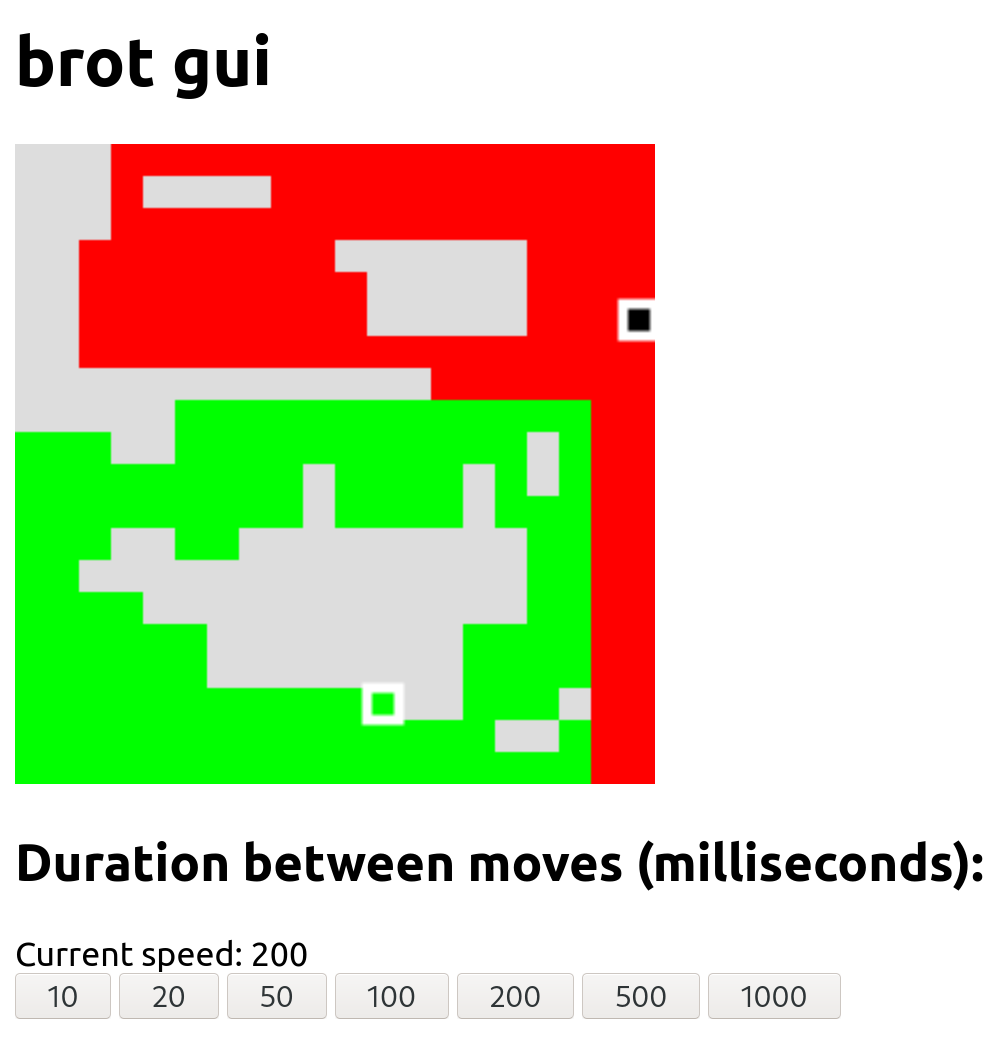
\includegraphics[width=0.6\textwidth]{gui.png}
    \caption{GUI während eines Spiels zwischen zwei Spielern der Combi Strategie}
    \label{fig:gui}
\end{figure}

\begin{figure}
    \centering
    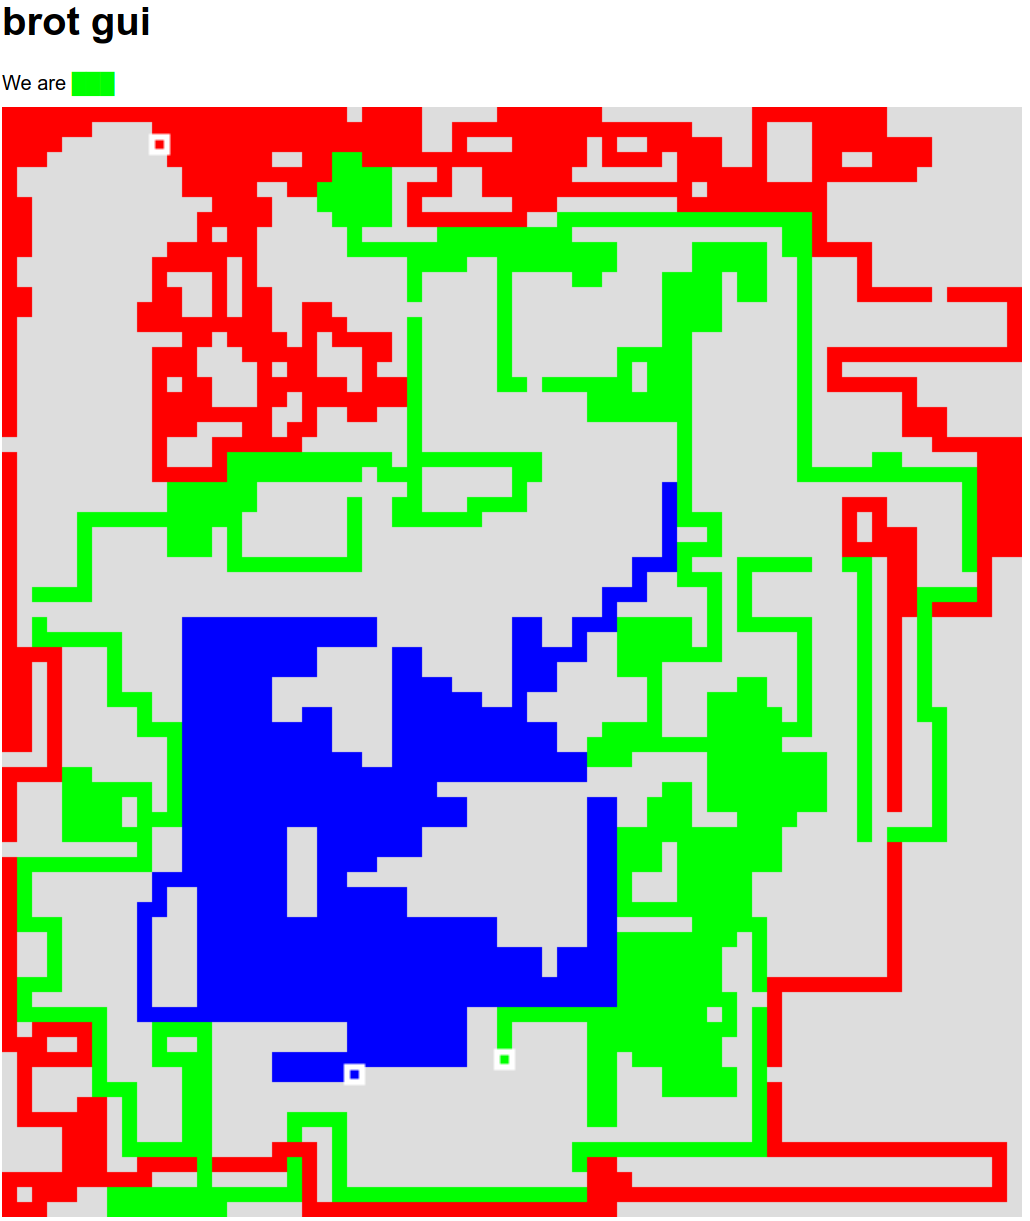
\includegraphics[width=0.6\textwidth]{gui2.png}
    \caption{GUI während eines Spiels auf der offiziellen API}
    \label{fig:guiAPI}
\end{figure}

Die Skripte bestehen aus Bash-Testskripten.  \texttt{test\_internal.sh} lässt mehrere unserer Clients gegeneinander spielen und legt die dabei gesammelten Daten in einer Ordnerstruktur ab. Jeder Ordner repräsentiert dabei ein gespieltes Spiel und enthält die Logs aller Clients im JSON-Format, sowie in zwei getrennten Verzeichnissen die Ausgabe der einzelnen Clients als Textdateien und Fehlermeldungen der einzelnen Clients als Textdateien. Außerdem wird im Ordner des Spiels eine Datei namens \texttt{GameInfo.txt} erstellt, die die verwendeten Spieler und deren Hyperparameter enthält. Dies ermöglicht die effiziente Analyse zusammenhängender Logs. Um das Skript zu benutzen, müssen die Parameter am Anfang des Skripts an die zu testenden Werte angepasst werden und es muss spezifiziert werden, wohin die Logdateien geschrieben werden. Das Skript erwartet keine Argumente. Das zweite Testskript heißt \texttt{test\_api.sh}. Dieses Skript startet das Programm in einer Endlosschleife, wobei alle Logdateien in ein Verzeichnis geschrieben werden. Das Skript erwartet keine Argumente, Umgebungsvariablen für den Client müssen jedoch trotzdem gesetzt werden.

Beide Bash-Skripte lassen sich beenden, indem im Projektverzeichnis eine Datei mit dem Namen \texttt{stop} erstellt wird. In diesem Fall wird kein neues Spiel gestartet.

Weiterhin gibt es zwei Python3-Auswertungsskripte mit denen Logs analysiert werden können. \texttt{visualize.py} wandelt ein JSON-Log in ein Video des Spielverlaufs um. Am Anfang eines jeden Videos werden Informationen über das Spiel angezeigt, wie der belegte Platz, der verwendete Server oder die Anzahl der gegnerischen Spieler. Das Skript erwartet als Argumente einen oder mehr Dateinamen von JSON-Logfiles des Clients. Zudem werden als Abhängigkeiten die Python-Pakete \texttt{Pillow} und \texttt{ffmpeg} sowie das Programm \texttt{ffmpeg}\footnote{Download: \texttt{https://ffmpeg.org/}, zuletzt aufgerufen: 17.01.2021} selbst benötigt.

Das Python3-Skript \texttt{stats.py} gibt Statistiken für gegebene Spiele in Textform aus, die den Spielerfolg in Abhängigkeit verschiedener Einflussfaktoren, wie der Hyperparameter, Anzahl an Spielern oder konkrete Gegner, aufschlüsseln. Das Skript hat keine Abhängigkeiten, jedoch wird das Paket \texttt{matplotplib} benötigt, falls Diagramme erstellt werden sollen. Seine Argumente sind durch \texttt{./stats.py --help} dokumentiert. Das Skript erwartet ein oder mehr JSON-Logfiles oder Ordnerstrukturen, die durch \texttt{test\_internal.sh} erstellt wurden als Argumente, sowie eine Information welche Statistiken erstellt werden sollen, z.B. \texttt{-a} für alle möglichen Statistiken. Das Skript kann für die Hyperparameter ein Diagramm erstellen.


\section{Hyperparameter}\label{sec:combi-hyperparameter}
Wie genau die unterschiedlichen Ansätze zusammenarbeiten, hängt von verschiedenen Hyperparametern ab. Um hierbei die besten Werte zu finden, haben wir ausführliche Tests durchgeführt (insgesamt mehr als 450 Spiele). Die Ergebnisse sind in Abbildungen \ref{fig:hyperparameters-1}, \ref{fig:hyperparameters-2} und \ref{fig:hyperparameters-3} zu sehen. Wir haben uns bei der Optimierung auf drei Hyperparameter beschränkt, die wir als zentral für das Spielverhalten ausgemacht haben, \texttt{myStartProbability}, \texttt{minimax\ ActivationValue} und \texttt{filterValue}. \texttt{myStartProbability} wirkt sich auf den Ansatz der Wahrscheinlichkeitstabellen aus. Normalerweise wird der erste Knoten im Baum mit der Startwahrscheinlichkeit 1.0 versehen. Ändert man diese für den eigenen Knoten, kann man entweder ein aggressiveres Verhalten erreichen, indem man den Wert erhöht, oder ein Passiveres, indem man den Wert kleiner als 1.0 wählt. Die anderen beiden Parameter sind in Abschnitt \ref{sec:rollouts} (\texttt{filterValue}) und Abschnitt \ref{sec:combi-evaluation} (\texttt{minimaxActivationValue}) erklärt. Um ein Optimum für die Parameter zu ermitteln, haben wir in vier Iterationen verschiedene Bereiche für die Parameter festgelegt und anhand der Gewinnrate ermittelt, wo das Optimum für die Parameter liegen könnte. Die letzte Iteration ist nicht mehr dargestellt, da sie keine signifikanten Erkenntnisse mehr lieferte. Leider konnten wir bei unserem Testverfahren nur gegen unseren eigenen Spieler testen, da auf dem offiziellen Server Spiele so lange dauerten, dass es nicht möglich war, eine ausreichend große Datenbasis zu erhalten. Für die erste Iteration haben wir den einzelnen Parametern einen großen Wertebereich mit nur einigen Stichproben gegeben, um grob abschätzen zu können, in welchem Bereich das Optimum der einzelnen Parameter liegt.



\subsection{Iteration 1}

\begin{figure}[h]
    \centering
    \includesvg[width=\textwidth]{hyperparameters1.svg}
    \caption{Gewinnhäufigkeit in Abhängigkeit verschiedener Hyperparameter, erste Testiteration}
    \label{fig:hyperparameters-1}
\end{figure}

Beim \texttt{filterValue} ist zu sehen, dass ein Maximum bei 0.7 liegt. Deshalb haben wir in der nächsten Iteration einen feiner abgestuften Bereich um 0.7 gewählt, um das Optimum genauer bestimmen zu können. Bei \texttt{myStartProbability} ist zu sehen, dass Werte kleiner 1.0 eher schlecht abschneiden, deswegen haben wir diese in zukünftigen Iterationen nicht mehr berücksichtigt. Ansonsten konnte keine Aussage über \texttt{myStartProbability} getroffen werden. Bei \texttt{minimaxActivationValue} ist zu sehen, dass das aktuell ermittelte Optimum am rechten Rand des Intervalls liegt. Deswegen haben wir für die zweite Iteration das Intervall nach rechts verschoben.

\subsection{Iteration 2}

\begin{figure}[h!]
    \centering
    \includesvg[width=\textwidth]{hyperparameters2.svg}
    \caption{Gewinnhäufigkeit in Abhängigkeit verschiedener Hyperparameter, zweite Testiteration}
    \label{fig:hyperparameters-2}
\end{figure}

Das Maximum bei 0.7 hat sich für \texttt{filterValue} erneut manifestiert. In der nächsten Testiteration haben wir einen noch kleineren Wertebereich um 0.7 genommen, um das Optimum weiter einzugrenzen. Bei \texttt{myStartProbability} gibt es zwei Spitzen um 1.0 und 2.2. Wir haben beschlossen, das Intervall und die Abstufungen beizubehalten und nur die anderen Werte einzuschränken, um so Wechselwirkungen zwischen den Parametern zu eliminieren. Der \texttt{minimaxActivationValue} bleibt bei seinem Maximum um 0.005. Wir haben deshalb begonnen, das Intervall kleiner zu ziehen.

\subsection{Iteration 3}

\begin{figure}[h!]
    \centering
    \includesvg[width=\textwidth]{hyperparameters3.svg}
    \caption{Gewinnhäufigkeit in Abhängigkeit verschiedener Hyperparameter, dritte Testiteration}
    \label{fig:hyperparameters-3}
\end{figure}

Bei dieser Testreihe lag das Maximum für \texttt{filterValue} bei 0.69 sehr knapp vor 0.71. Wir haben deshalb 0.69 als \texttt{filterValue} für unsere Spiele auf der API festgesetzt. Bei der dritten Testreihe war ein Maximum von 1.2 für \texttt{myStartProbability} zu sehen. Für unsere ersten Tests auf der API haben wir deshalb diesen Wert gesetzt. Das Maximum lag bei der dritten Iteration bei 0.001 für \texttt{minimaxActivationValue}, sodass dieser Wert gewählt wurde.

\subsection{Manuelle Analyse}
Wir rechneten bereits damit, dass unsere Ergebnisse nur eine Annäherung für die API sein können. Je nach Gegenspieler sind sehr unterschiedliche Parameter optimal. Außerdem beeinflusst die Änderung eines Parameters auch das Optimum eines anderen Parameters. Deswegen haben wir das Spielverhalten unseres Clients auch qualitativ anhand von Logs und Visualisierungen des Spielverlaufs analysiert. Anschließend haben wir ähnliche Situationen, in denen suboptimale Entscheidungen getroffen wurden, nachgestellt und die Parameter so angepasst, dass Combi in der Situation nach der Anpassung besser handelt. Der \texttt{filterValue} hat sich dabei nicht geändert und liegt weiterhin bei 0.69. Auch den Wert für \texttt{minimaxActivationValue} beließen wir, \texttt{myStartProbability} hoben wir jedoch auf 2.0 an.

\section{Auswertung}

\subsection{Intern}\label{sec:interne-evaluation}

Um zu verifizieren, dass der Combi-Client auch die effektivsten Strategien von all unseren Ansätzen verwendet, führten wir Testreihen auf einem lokalen Server (s. Kapitel \ref{sec:software-server}) durch. Dabei ließen wir in jeder Testreihe jeweils einen Combi-Client gegen einen Client einer anderen Strategie antreten und erfassten, wie viele der Spiele von welchem Client gewonnen wurden. In Abbildung \ref{fig:internal-testing} sind die Ergebnisse dargestellt.

\begin{figure}[h!]
    \centering
    \includesvg[width=0.7\textwidth]{chart_internal_testing.svg}
    \caption{Gewinnrate verschiedener Clients gegen Combi ($n \geq 100$ Spiele)}
    \label{fig:internal-testing}
\end{figure}

In der Abbildung sieht die jeweiligen Gewinnraten für die Spieler in den verschiedenen Spielerkombinationen. Der Wert wird ermittelt, indem die Anzahl an gewonnenen Spielen ins Verhältnis zur Gesamtanzahl der Spiele ($n$) gesetzt wird. Für jede Testreihe wurden dabei knapp über 100 Spiele durchgeführt, um die Gewinnrate als Vergleichswert nutzen zu können.

Der Basic-Client schneidet insgesamt am schlechtesten ab. Dieses Ergebnis war zu erwarten, da er die einfachste Logik nutzt und viele Faktoren nicht beachtet, die von den anderen Clients, insbesondere von Combi, berücksichtigt werden. Der MiniMax-Client und der Client, der die Wahrscheinlichkeitstabellen als Strategie nutzt, erreichen mit einer Gewinnrate von ca. 0.12 beide ein ähnliches Ergebnis. Der Rollout-Client schneidet insgesamt am besten von allen Strategien gegen den Combi-Client ab. Dieses Ergebnis weist auch auf die Bedeutung der Rollouts als Teil der Combi-Strategie hin, zeigt aber auch, dass Wahrscheinlichkeitstabellen und MiniMax Combi zu einem stärkeren Spieler machen, als es Rollouts ursprünglich sind. Insgesamt ist deutlich erkennbar, dass der Combi-Client den anderen Strategien in jedem Fall deutlich überlegen ist.
 
\subsection{Offizielle API}
Um die Qualität unseres Ansatzes bewerten zu können, haben wir Combi lange auf dem offiziellen Server getestet.
Natürlich wäre es wünschenswert gewesen, dies für alle Strategien tun zu können, jedoch konnten wir mit unserem API-Key nur ein Spiel gleichzeitig spielen und Spiele dauerten teilweise mehrere Stunden, sodass die Anzahl an Testspielen stark begrenzt war. Dementsprechend wollten wir diese begrenzte Kapazität darauf verwenden, aussagekräftige Daten über Combi zu sammeln.

\begin{figure}[h]
    \centering
    \begin{tabular}{l|r|r|r}
        Client & Gespielte Spiele & Gewonnene Spiele & Gewinnhäufigkeit \\ \hline \hline
        Combi & 100 & 83 & 0.830 \\ \hline
        Combi (bereinigt) & 79 & 63 & 0.797 \\ \hline
        Basic & 16 & 2 & 0.125 \\
    \end{tabular}
    \caption{Gewinnhäufigkeit verschiedener Clients auf der API}
    \label{fig:api-testing}
\end{figure}

Insgesamt haben wir 100 Spiele auf der API absolviert und davon 83 gewonnen. Um eine bessere Einschätzung unserer tatsächlichen Gewinnrate zu erhalten, haben wir die Daten manuell bereinigt, indem wir Spiele entfernt haben, in denen die Gegner innerhalb weniger Züge ohne unser Eingreifen oder aufgrund von Timeouts gestorben sind. Nach der Bereinigung bleiben noch 79 Spiele übrig, von denen wir 63 gewonnen haben. Das ergibt eine Gewinnrate von ca. $79,7\%$ Diese ist jedoch nicht sehr aussagekräftig für die Qualität der Lösung gegen spezifische Clients. Die Gewinnrate zeigt also nur die Qualität unserer Lösung im Vergleich zu anderen Teams, die zum gleichen Zeitpunkt wie wir viel getestet haben und gegen deren Spieler wir ungefähr gleich oft angetreten sind. Nichtsdestotrotz ist eine Gewinnrate von fast 80\% gut, wenn man davon ausgeht, dass bei einem \texttt{spe\_ed}-Spiel mit 2 bis 6 Spielern die zufällige Gewinnchance bei $\frac{1}{6}$ bis $\frac{1}{2}$ liegt.

Unsere Gewinnrate (bereinigt) schwankte kaum abhängig von der Anzahl an Spielern, wie in Abbildung \ref{fig:api-num-players} zu sehen ist. Aus den Daten lässt sich folgern, dass Combi auch mit vielen Spielern zurechtkommt.

\begin{figure}[h]
    \centering
    \includesvg[width=\textwidth]{chart_success_by_num_players.svg}
    \caption{Analyse der API-Ergebnisse nach Anzahl an Spielern}
    \label{fig:api-num-players}
\end{figure}

Um zu überprüfen, wie unser Ansatz gegen spezifische andere Spieler zurechtkommt, haben wir aufgeschlüsselt, gegen welche Pseudonyme wir überhaupt verloren haben und wie die Gewinnrate gegen diese Pseudonyme aussieht (Abbildung \ref{fig:pseudonyme}). Pseudonyme werden vom Server am Ende eines jeden Spiels angegeben und identifizieren einen Client über einen gewissen Zeitraum eindeutig. Unsere Analysen haben ergeben, dass unser Pseudonym zumindest über mehrere Tage gleichblieb. Bei dieser Auswertung wird deutlich, dass der Unterschied zwischen einzelnen anderen Spielern sehr drastisch ist. Im Extremfall konnten wir nur 25\% der Spiele für uns entscheiden, gegen andere Spieler hingegen über 90\%. Spieler gegen die wir 100\% der Spiele für uns entscheiden konnten, haben wir nicht in der Tabelle aufgeführt. Dies waren 35 von 43 Pseudonymen, gegen die wir gespielt haben. Die Spiele mit dem Gegner, gegen den wir nur 25\% aller Spiele gewonnen haben, bieten eine geringe Datenbasis, dennoch haben wir die Spiele qualitativ analysiert. Uns fiel auf, dass sich sein Spielverhalten von anderen Gegnern vor allem dadurch unterscheidet, dass er sehr aggressiv spielt und ständig versucht, unserem Spieler den Weg abzuschneiden. Trotzdem könnte man wahrscheinlich eine bessere Gewinnrate erreichen, indem man sein spezifisches Spielverhalten analysiert und die Hyperparameter anpasst, zum Beispiel indem \texttt{myStartProbability} niedriger gesetzt wird, damit unser Spieler noch defensiver spielt.

\begin{figure}[h]
    \centering
    \begin{tabular}{r|r|r|r}
        Spieler & Gespielte Spiele & Gewonnene Spiele & Gewinnhäufigkeit \\ \hline \hline
        1 & 18 & 15 & 83.3\% \\ \hline
        2 & 5 & 4 & 80.0\% \\ \hline
        3 & 24 & 23 &  95.8\% \\ \hline
        4 & 4 & 1 & 25.0\% \\ \hline
        5 & 4 & 3 & 75.0\% \\ \hline
        6 & 11 & 10 & 90.9\% \\ \hline
        7 & 4 & 3 & 75.0\% \\ \hline
        8 & 6 & 4 & 66.7\% \\
    \end{tabular}
    \caption{Gewinnhäufigkeit gegen Clients, gegen die mindestens ein Spiel verloren wurde}
    \label{fig:pseudonyme}
\end{figure}

In Zeiten, als wir die API nicht genutzt haben, haben wir den Basic-Client auf der API spielen lassen um eine Referenz zu haben, wie ein simpler Ansatz auf der API abschneidet. Der Basic-Client konnte unbereinigt 2 von 16 Spielen für sich entscheiden. Dies entspricht einer Gewinnrate von 12,5\%. Obwohl die Datenbasis mit 16 gespielten Spielen sehr gering ist, lässt sich sagen, dass der Combi-Client im Vergleich dazu mit einer unbereinigten Gewinnrate von 83\% deutlich besser abschneidet.


\section{Diskussion}
Das Spiel \texttt{spe\_ed} ist sehr komplex. Die von uns betrachteten Strategien können einzeln nicht alle spezifischen Eigenschaften des Spiels abdecken. Erst durch die Kombination mehrerer Strategien im Combi-Client können die meisten Herausforderungen überwunden werden. Wie unsere Testergebnisse zeigen, ist der Combi-Client erfolgreicher als jede der beteiligten Ansätze alleine (siehe Abschnitt \ref{sec:interne-evaluation}). Auch gegen andere Teams konnte unser Client eine beachtliche Anzahl von Spielen gewinnen (mehr als 80\%). Allerdings ist das Potenzial unserer Lösung noch nicht vollständig ausgeschöpft. Denn sowohl die einzelnen Strategien, als auch ihre Kombination bieten noch Raum für Verbesserungen.

\subsection{Verbesserungen MiniMax}
MiniMax bewertet eine Spielsituation anhand des Freiheitsgrades unseres Spielers. Diese Heuristik fokussiert sich lediglich auf die eigenen Überlebenschancen und vernachlässigt dabei den Einfluss unseres Handelns auf die Überlebenschancen des Gegners. Da es jedoch nur darauf ankommt, als letzter Spieler aktiv zu sein, wäre es durchaus sinnvoll, dies in die Betrachtung mit einzubeziehen. Wenn zum Beispiel nur noch ein anderer Spieler aktiv ist, bedeutet sein Ausscheiden unseren sicheren Sieg. Es ist jedoch schwierig, dafür eine passende Heuristik zu entwickeln, die nicht dafür sorgt, dass wir ein zu hohes Risiko eingehen und dadurch ausscheiden. Außerdem ist es schwierig zu bewerten, ob ein anderer Spieler durch unseren Zug ausscheidet oder ihm sowieso keine Möglichkeiten mehr bleiben. Diese Schwierigkeit ist besonders groß, wenn noch mehrere Spieler am Leben sind.

\subsection{Verbesserungen Rollouts}
Die Rolloutstrategie wählt in ihrer aktuellen Implementierung Züge absolut zufällig aus. Dadurch kann es passieren, dass Pfade mehrmals überprüft werden. Dies bedeutet, dass die Berechnungszeit effizienter genutzt werden könnte, denn mehr verschiedene Rollouts bedeuten, dass die Heuristik einen besseren Gesamtüberblick gibt. Denkbar wäre ein Ansatz der mit einer Tiefensuche den Spielbaum aufbaut. Dabei wird durch jeden Rollout der Spielbaum erweitert. Ein Blatt im Baum ist dann immer ein Spielzustand in dem es keine weiteren Züge für unseren Spieler gibt. Fraglich ist, ob diese Methode speichereffizient implementiert werden kann und der Verlust an Geschwindigkeit durch weniger mehrfach ausgeführte Pfade kompensiert werden kann.

\subsection{Verbesserungen Wahrscheinlichkeitstabellen}
Aktuell nehmen wir für die Wahrscheinlichkeitstabellen an, dass jeder mögliche Zug mit gleicher Wahrscheinlichkeit ausgeführt wird. Dies entspricht nur selten dem eigentlichen Spielgeschehen. Wenn ein Spieler in einem langen Zeitraum seine Geschwindigkeit nicht verändert hat, könnten beispielsweise die Wahrscheinlichkeiten für die Züge \texttt{speed\_up} und \texttt{slow\_down} herabgesetzt werden. In diesem Fall wählt unser Spieler eine zu passive Strategie anhand der Wahrscheinlichkeitstabellen. Letztendlich haben wir uns vorerst gegen eine solche Anpassung entschieden. Der Hauptvorteil der Wahrscheinlichkeitstabellen ist, dass das Spielgeschehen ganzheitlich abgebildet wird. Eine falsche Vorhersage über das Spielverhalten der Gegner könnte diesen Vorteil zunichtemachen.

\subsection{Verbesserungen Combi}
Das Verhalten des Clients hängt maßgeblich von den verschiedenen Hyperparametern ab. Diese haben wir versucht, durch interne Tests und Beobachtungen auf der API zu verbessern (\ref{sec:combi-hyperparameter}). Allerdings haben wir uns bei der Optimierung nur auf drei Hyperparameter beschränkt, um aussagekräftige Daten sammeln zu können. Um Verbesserungen zu erzielen, sollten weitere Hyperparameter eingeführt werden. Obwohl bereits bei der jetzigen Optimierung nicht alle Hyperparameter berücksichtigt werden konnten, könnte es sinnvoll sein, einen Hyperparameter für die Gewichtung zwischen Rollouts und Wahrscheinlichkeitstabellen einzuführen. Dieser Wert würde die Risikobereitschaft unseres Spielers steuern.

Zudem haben wir festgestellt, dass es schwierig ist, optimale Werte für die verschiedenen Hyperparameter durch Tests zu ermitteln. Deshalb wäre es sinnvoll, die Werte dynamisch an die Spielsituation und das Verhalten der Gegner anzupassen. Dies ist jedoch nicht trivial, da man Kriterien finden müsste, anhand derer die Spielsituation zuverlässig bewertet werden kann. 

Neben der Anpassung von Hyperparametern, könnte eine gänzlich andere Auswertung zu weiteren Verbesserungen führen. Nach aktueller Implementierung werden meistens sehr passive Züge gewählt. Bei der Auswertung von Rollouts, Wahrscheinlichkeitstabellen und den Ergebnissen von MiniMax wird stets versucht, die eigene Überlebensdauer zu maximieren. Ähnlich wie bei MiniMax, wird dabei vernachlässigt, dass auch ein Ausscheiden des Gegners für uns von Vorteil ist. Mit einer veränderten Auswertung, die dies berücksichtigt, wäre ein aggressiveres Spielverhalten möglich. Der Combi-Client könnte versuchen, andere Spieler einzukesseln oder ihnen den Weg abzuschneiden.

\subsection{Integration von Machine Learning}
Die Wahrscheinlichkeitstabellen geben eine Spielsituation sehr gut wieder. In dieser sind nämlich indirekt Position, Geschwindigkeit und Bewegungsrichtung der anderen Spieler enthalten. Man könnte diese daher als Eingabevektor für ein neuronales Netz benutzen und davon den aktuell besten Zug bestimmen lassen. Problematisch dabei ist, dass die Berechnung der Wahrscheinlichkeitstabellen, die gesamte Berechnungszeit in Anspruch nimmt. Man könnte deshalb für den aktuellen Zug immer nur auf die Wahrscheinlichkeitstabellen des letzten Zuges zurückgreifen. Es ist fraglich ob dies ein zu großer Nachteil für den Spieler, der nach dieser Strategie spielt, wäre oder ob er trotz dieses Nachteils das Spiel gut erlernen könnte. Neben der Besuchswahrscheinlichkeit für andere Spieler wäre auch problemlos möglich einen zweiten Eingabevektor zu errechnen, der angibt wie wahrscheinlich es ist, dass unser Spieler eine Zelle besuchen kann.

\subsection{Übertragung auf andere Probleme}
Bei näherer Betrachtung von Combi wird schnell deutlich, dass dieser sehr spezifisch für das Spiel \texttt{spe\_ed} implementiert ist. Allerdings können die einzelnen Komponenten, wie die Wahrscheinlichkeitstabellen oder die Herangehensweise der Rollouts, durchaus übertragen werden. Auch die Analyse und Auswertung könnten Anwendung finden, auch außerhalb von automatischen Spielen.

\section{Fazit}
Insgesamt erzielt der beschriebene Ansatz mit seinem aktuellen Satz an Parametern sehr zufriedenstellende Ergebnisse. Durch das Ändern der Hyperparameter lässt sich das Spielverhalten maßgeblich beeinflussen. Unsere Lösung ist wandelbar und kann durch minimale Anpassungen an spezifische Anforderungen angepasst werden. Die Software ist einfach erweiterbar: Zusätzlich zur modularen Client-Implementierung haben wir mit unserem Server, der GUI und den Test- und Auswertungsskripten einen Rahmen geschaffen, der die einfache Umsetzung und Analyse neuer Spielansätze ermöglicht.

%===========================================================
%===========================================================

\bibliographystyle{ieeetr}
\bibliography{refs}


\end{document} 

